%!TEX root = article.tex

%%%%%%%%%%%%%%%%%%%%%%%%%%%%%%%%%%%%%%%%%%%%%%%%%%
\section{Introduction}
\label{s:Introduction}

\subsection{Motivation}
%Why do we do this at all ?

This thesis aims to understand and specify how blood flow and oxygen transport has been simulated until today. The goal is to see how far existing methods, especially the Green's Function Method applied to this field by Secomb et al. \cite{Secomb2004} can produce accurate results for new and especially complex networks. A new model using an open source software called $DuMu^x$ \cite{flemischdumux} was implemented to offer a different approach for oxygen transport and diffusion simulations.\\
\\Oxygen from blood is carried on to the tissue of living organs through a
complex network of vessels, in particular by capillaries that provide oxygen to
the tissue, which is attached to the red blood cells. 
The complex biochemistry involved in the release of oxygen from hemoglobin and
its transport to the surrounding tissue is a complex process that cannot be
fully understood by experimental methods.
With the advent of mathematical models and advanced computing architectures,
the process of Oxygen delivery to the tissue can be simulated to understand
various physiological and pathophysiological processes.\\
\\This thesis aims to simulate transport of oxygen through capillary networks of
various organs using mathematical models.
Specifically, the goal is to evaluate the efficacy of the existing numerical
methods that simulate flow and transport of $O_2$ through capillaries.
The Green's function method developed by Secomb is evaluated in detail and
applied to various microvasculature networks.
Further, coupling of 1D network with a 3D surrounding tissue is evaluated in
the open source package called $DuMu^x$.
A simplified approach for the simulation of $O_2$ transport was implemented in
 $DuMu^x$ and compared with the results of Green's function method.

\subsection{Structure of the Thesis}
%This thesis will have following structure ...

First, a short insight to the physiological background of blood flow and oxygen transport in the body will be given.The general process of oxygen delivery to the tissue and oxygen consumption by the tissue will be explained. The main subject will be the transport of oxygen in the body, starting in the blood flow and ending in the diffusion into the tissue through a general diffusion process.
\\The results of oxygen transport simulation methods, especially the Green's Function Method, will later be discussed and evaluated for different networks. In addition to this, a new oxygen delivery model was implemented using an open source software called $DuMu^x$. The focus of this thesis is to understand when and why the Green's Function Method produces physiologically accurate results, how it can perform on new networks and compare these results to alternatives such as the implemented method on $DuMu^x$.

%%%%%%%%%%%%%%%%%%%%%%%%%%%%%%%%%%%%%%%%%%%%%%%%%%
\newpage
\section{Blood Flow and Oxygen Delivery}
%How does this work physiologically ?

In this section the physiological aspects of $O_2$ transport through vessels into the tissue will be discussed. This part is mainly dedicated to the understanding of physical processes that are involved in the transport of oxygen through capillaries into the tissue, and its consumption therein. The ultimate goal of this research topic in the Interface Group is to understand the production of EPO and the physiologic phenomenon behind an increased EPO production. The main idea is to compute oxygen concentration fields in the kidney, where local hypoxia generally leads to an EPO emission. ({\color{red}mention this or rather not?})
\\To give the reader a short overview, I will start at the beginning and give a brief explanation of how blood travels through the body. How it is pumped through the heart into the whole body, carrying well oxygenated fresh blood from the heart to the tissues everywhere in the body, and then back from the tissues to the heart through the veins.
\\In this thesis, the flow and transport through micro-vessels in the capillary range and in the tissue is the main concern, where generally the time-dependency of the blood-velocity will not be taken into account. The periodic beating of the heart causes the velocity to be inconstant, but this effect can be neglected for modeling purposes and computations, as it's rather irrelevant. For this, we will use a steady-state approximation for the flow rate, and thus assume a constant velocity. This means that there is no variation of velocity depending on time for any given point in the network.

\subsection{Blood Flow}
\label{Blood Flow}
%Purely physiological Blood Flow part (with mathematical formulas to describe processes)
%Discuss General Hemodynamics
%Put some papers and references in and explain some values and parameters.
%Use mathematics paper for blood flow calculations \cite{mathmodeling}
%Papers to cite: \cite{pittman2011regulation}
%Explain this in a bit more detail. 
%Also mention that blood is usually modeled as a homogeneous fluid using Navier Stokes equations despite that it is a mixture of plasma and cells etc.
%Also mention that why it is extremely inappropriate for us to model it like that.

Blood is basically composed of two phases: liquid and cells. The liquid phase is called plasma, and the cells that play the most important role for our concern are the red blood cells. This will later be important when considering the oxygen transport in the blood. For computational models, blood is generally modeled as an incompressible Newtonian fluid \cite{mathmodeling}. This basically means that the viscous stress is linearly proportional to the strain rate. Modeling blood as a Newtonian fluid is basically a wrong assumption, due to the fact that only the plasma is a Newtonian fluid. Nevertheless, this model of blood is used a lot as it can produce fairly good results and for the fact that taking irrelevant details into account wouldn't be very interesting for oxygen transport simulations {\color{red} (can I say it like this ?)}. It is also important to mention that the cells, making up to 40-45\% of the blood volume, are basically not incompressible. They can be compressed and might even shrink in order to facilitate the blood flow in small vessels.
\\While our model of blood uses big assumptions and turns a two phase medium into an incompressible Newtonian fluid, this immensely facilitates computations from an engineering point of view and can produce fairly good results.
Using this model for blood leads to the Navier-Stokes equations \ref{eq:NavierStokes1}, \ref{eq:NavierStokes2}, which basically describe the flow dynamics of an incompressible Newtonian fluid:
\begin{equation}
\\ \rho \frac{\delta \textbf{v}}{\delta t} + \rho \textbf{v} \nabla \textbf{v} + \nabla p - \eta \nabla ( \nabla \textbf{v} + \nabla \textbf{v}^T ) = \textbf{f}
\label{eq:NavierStokes1}
\end{equation}
\begin{equation}
\\ \nabla \textbf{v} = 0
\label{eq:NavierStokes2}
\end{equation}
In the Navier-Stokes equations, $\textbf{v}$ is the velocity vector, $p$ is the pressure, and $\rho$ and $\eta$ are the blood density and viscosity respectively.
\\The external forces acting on the fluid are represented by the vector $\textbf{f} = (f_x f_y f_z)^T$.
\\The first and the second term on the left-hand side are corresponding to inertial forces, while the third term stands for the pressure force and the fourth term for the viscous force. The sum of these forces must be equal to the right-hand side, where we only have the external forces \textbf{f}.
\\The next step in order to solve these equations for the blood flow in a given vessel is to put appropriate initial and boundary conditions. An example of useful boundary conditions is given here:
\\\begin{equation}
\\ \textbf{v}_{in} =  \textbf{v}_0
\label{eq:Boundary1}
\end{equation}
\begin{equation}
\\ \textbf{v}_{vessel wall} =  0
\label{eq:Boundary2}
\end{equation}
\\Here we put the velocity $\textbf{v}_{in}$ of the fluid entering our domain equal to a velocity vector $\textbf{v}_0$ and prescribe a non-slip condition on the vessel walls. Solving the Navier-Stokes equations \ref{eq:NavierStokes1}, \ref{eq:NavierStokes2} using appropriate initial conditions and making a few other assumptions will then lead to the Poiseuille-Flow which can generally be used to describe Newtonian fluid flows in pipes.
\\ {\color{red} (hey kartik, are the explanations here good enough ? you said I should keep this part short, so please give me a feedback if this gives a good enough insight to the flow and if everything is correct)}

\subsection{Oxygen Transport and Delivery}
%Purely physiological Oxygen part (with mathematical formulas to describe processes)
%How does this oxygen related stuff physically and physiologically work ?
%\\Again put some papers and references in and explain some physical diffusion equations, values and parameters.
%\\Why do we care about this etc. ?
%\\Diffusion, Parameters, etc. etc.
%\\Use Vasomotion paper for oxygen delivery \cite{goldman2001computational}
%\\Papers to cite: \cite{bukwirwa}

Through breathing, oxygen enters the body and fills the lungs. As gases tend to move from areas with higher concentrations towards areas with lower concentrations, oxygen moves from the oxygen rich air towards the alveoli and enters the blood \cite{bukwirwa}. This same concentration gradient will later transport the oxygen into the tissue during the diffusion process. The physical processes behind this will briefly be explained in this section.

\subsubsection*{Oxygen Transport in the Blood}
%Transport with the flow
%Binding of Oxygen to Red Blood Cells
%Oxygen Concentration etc.
%Papers to cite: \cite{hellums1977resistance}.
%Plasma and Red Blood Cells
%Hemoglobin

As mentioned in the previous chapter, blood is composed of plasma and red blood cells. The red blood cells are the main carriers of oxygen in the blood \cite{pittman2011regulation}. In this section, we will mainly focus on the red blood cells, as these are the main oxygen carriers. As the general concern of this thesis is not the physiological oxygen-red blood cell interaction, I will just briefly explain the basic principle behind oxygen transport in the blood.
\\The oxygen carrier contained in the red blood cells is called hemoglobin. Hemoglobin is a protein which can chemically bind oxygen molecules. This means that while our blood travels through the vessels, oxygen is supplied to every cell in the body by the hemoglobin which binds oxygen and transports it with the blood flow.

\subsubsection*{Oxygen Diffusion Into the Tissue}
%Diffusion out of the Vessels - Fick's Law of Diffusion
%Diffusion Process - Transport in the Tissue - Properties and some general Parameters
%Delivery of Oxygen to the Cells
%Papers to cite: \cite{hellums1977resistance}, \cite{bukwirwa}

As previously mentioned, diffusion will play an important role for oxygen transport in the body. This is due to the fact that diffusion is the principle physical mechanism of how oxygen from the vessels is reaching the tissue. Without diffusion, oxygen would basically never penetrate the tissue and would only travel the body like in a closed loop circuit. This physical phenomenon is described by Fick's Law of Diffusion:
\begin{equation}
\\J = - D \frac{dc}{dx}
\label{Fick}
\end{equation}
Where J is the diffusive flux, D is the previously mentioned diffusivity coefficient, and $\frac{dc}{dx}$ is the derivative of the concentration with respect to the distance x, which is the concentration gradient \cite{pittman2011regulation}, \cite{lee2017accounting}.
\\The diffusion process can be helped and enhanced by a substance (molecule?) called Myoglobin. This substance can be found in some tissues in the body, especially muscle tissue (?) and enhances the diffusivity of oxygen through the tissue. The enhancement effect can depend on the Myoglobin concentration in the given tissue, and these effects can be taken into account by (?). \cite{wittenberg1970myoglobin}


\subsection{Current Trends in Modeling}
%Use a few papers to give examples for previous and actual approaches
%Do link to modeling and models in this field in general, then link this to computational models in this field and their use. Actual trends and what people hope for in the future (in terms of computational power, computational methods but also from a medical perspective) is also interesting.
%Papers to cite: \cite{mathmodeling}, \cite{goldman2001computational}, \cite{kuzmin2010guide}, \cite{lee2017accounting}, \cite{beard2001modeling}, \cite{Secomb2004}

In order to simulate flows, Computational Fluid Dynamics (CFD) is a tool that can be used to produce results which can not be obtained through in vitro or in vivo experiments  \cite{mathmodeling}. For this reason and because the computational capabilities available are growing everyday, modeling and simulating processes in the body is taking an increasingly important role in biological and medical sciences.
\\In our case, the focus will lie on oxygen transport simulations and their computational implementation.\\
\\As already mentioned in the section \ref{Blood Flow}, blood flow in the body can be approximated by the Navier-Stokes equations \ref{eq:NavierStokes1}, \ref{eq:NavierStokes2}. The transport of oxygen in the blood can then be linked to this by the transport equations. These physical equations are quite straightforward to implement and solve numerically. The next task remains the biggest problem in actual research: Link this transport to the diffusion process out of the vessels and into the tissue. The biggest problems here seem to be in choosing the right/appropriate boundary conditions to get exact results. Also, many numerical methods fail or more specifically become unstable when the vessel network becomes complicated and heterogeneous. There are already good methods to produce results for the Krogh model, but to compute oxygen fields in very complex networks like in the kidney, these models do not provide the desired results.
\\Steady-State approximation for simulations: Need this assumption for Michaelis-Menten relation.


%In each of your categories (or subcategories if your topic is
%broad), we would like the following three points to be developed:
%\begin{enumerate}
 %   \item Concepts, definitions, value
%of this topic etc. For explanations that do not really fit in the
%text you may want to use footnotes\footnote{footnotes are shown
%below like this.} or by using the appendix (e.g. "see appendix
%\ref{s:ExtraStuff}").
 %   \item State of the art, discussing the work in the field, etc. E.g. Shaninpoor et al. \cite{shaninpoor98} have shown that ...
 %   \item Outlook: where do you feel this field is going. How would you continue your research on this
  %  topic?
%\end{enumerate}


%%%%%%%%%%%%%%%%%%%%%%%%%%%%%%%%%%%%%%%%%%%%%%%%%%
\newpage
\section{Simulation Methods}
%Everything about the computations behind the simulations and all I did.

As noted before, this thesis focuses on the evaluation of existing
methods that simulate flow and oxygen transport in micro-vasculature networks
and applies them to several vasculature morphologies from various organs. In this section I will try to give an overall understanding to the theoretical background to the Green's Function Method and accordingly the code developed by Secomb et al. \cite{Secomb2004}. Later on I will present a new model that I implemented using $DuMu^x$. Both the methods and the produced results will be discussed in the following sections.

\subsection{Green's Function Method}
%Here I will talk about everything concerning the Green's Method Code.

The Green's Function Method was first used for numerical computations of oxygen delivery in the tissue by Secomb et al. \cite{Secomb2004}. It can deliver accurate results with lower computational cost when compared to implicit methods, due to the fact that the number of unknowns is reduced. For simple networks like the examples specified in the next chapter, the method seems to be stable and produce accurate results. However, using new and more complex networks, the Green's Function Method seems to produce bad results and shows characteristics of unstability (at least we think so for now). As the results get bad, the computational advantages of this method are not of any use (bad formulation?).
\\The mathematical background behind the Green's Function Method and the numerical method derived from it will be discussed in the upcoming section. The accuracy of produced results as well as the physiological meaning behind these results will be the main subject in this chapter.

\subsubsection{The Computational Model}
%Just mathematical theory behind this method

General explanation about Green's Method code and how it works, especially mathematics behind the Green's Function Method (many mathematical formulas) and why it makes sense to use this. Also especially why is this interesting in physiological applications and oxygen delivery/consumption simulations ?
\\Goals:
\\- Avoid no flux boundary condition
\\- Find a systematic method that can be applied to tissue domains of arbitrary shape
\\- Find a cheap solution in terms of computational cost (when compared to implicit methods)
\\- Green's function method is computationally less expensive than the implicit methods, due to the fact that there is a lower number of unknowns

%\subsubsection*{The Computational Model}
%Methods and physiological assumptions used in this model.
%Very useful to use Governing Equations section of Secomb here

In this subsection, the used physical quantities, the assumptions and governing equations will briefly be explained. The equations cited here are, in my opinion, the most important ones to describe the physical background for the treated problem. This part strongly relies on the description by Secomb et al. \cite{Secomb2004}.
\\When looking at the code of the Green's Function Method, and especially at the inputs \ref{Inputs}, one can see that the tissue is modeled as a homogeneous medium. This results in constant oxygen diffusivity and solubility coefficients D and $\alpha$ respectively. These quantities usually have to be specified in the SoluteParams.dat-file. A more detailed explanation to the Inputs can be found in the Inputs section \ref{Inputs}.
\\The governing equations are listed here, with a short explanation for each of them:
\\As previously described, diffusion will play an important role in oxygen transport in the body, as oxygen is reaching the tissue by diffusing out of the vessels. This physical phenomenon is described by Fick's Law of Diffusion \ref{Fick}.
%
As a reminder, I want to mention that Fick's first Law gives the diffusive flux, which we are interested in, as a function of the diffusivity and the concentration gradient in the tissue.
\\In addition to this, the principle of conservation of mass applies to oxygen, and we have:
\begin{equation}
\frac{\delta \rho} {\delta t} + \nabla (\rho v) = 0
\end{equation}
%
These two fundamental equations can be combined to finally get:
\begin{equation}
\\D\alpha\nabla^2P = M(P)
\label{eq:DiffusionEq}
\end{equation}
%
\ref{eq:DiffusionEq} describes the dependency between the oxygen partial pressure P and the consumption rate M(P). Here I would like to mention the fact that partial pressure is physically nothing else than the concentration used in \ref{Fick}.
For the consumption, a Michaelis-Menten relationship applied to the problem is used:
\begin{equation}
\\M(P) = \frac{M_0P}{(P_0 + P)}
\label{eq:MichaelisMenten}
\end{equation}
%
In \ref{eq:MichaelisMenten}, M(P) is the consumption, $M_0$ the demand and $P_0$ the partial pressure at half-maximal consumption.
\\As previously mentioned, the second important physical phenomenon to describe our transport problem is the convective transport in the blood flow. To model this, we need to know the rate of convective oxygen that is transported through a single vessel segment.
\begin{equation}
\\f(P_b) = Q(H_DC_0S(P_b) + \alpha_{eff}P_b)
\label{eq:ConvTrans}
\end{equation}
%
In \ref{eq:ConvTrans}, the flow rate of blood is Q, and $H_D$, S, $C_0$, $P_b$ and $\alpha_{eff}$ are parameters such as discharge hematocrit, oxyhemoglobin saturation or partial pressure of oxygen in the blood. (Here specify everything yes or no ? Maybe use a symbols table at beginning to make things easier).
\\The previously mentioned oxyhemoglobin saturation can be computed by Hill's equation:
\begin{equation}
\\S(P_b) = \frac{P_b^n}{(P_b^n+P_{50}^n)}
\label{eq:Hill}
\end{equation}
In Hill's equation \ref{eq:Hill}, $P_b$ ist the previously mentioned partial pressure of oxygen in blood, $P_{50}$ is the partial pressure of oxygen at 50\% saturation and n is a constant.
%
\\Another important equation that we need to describe the given problem is the relationship describing the rate of of diffusive oxygen efflux per unit vessel length:
\begin{equation}
\\ \frac{df(P_b)}{ds} = -q_v(s)
\label{eq:ConsOxygen}
\end{equation}
\ref{eq:ConsOxygen} is obtained by using the conservation of oxygen along a vessel segment.
%
\\The continuity condition for the partial pressure of oxygen on the vessel-tissue interface gives a second equation for the diffusive oxygen flux:
\begin{equation}
\\q_v(s) = -D\alpha \int_{0}^{2\Pi} 
\frac{\delta P}{\delta r}r_v d \Theta
\label{eq:DiffFlux}
\end{equation}
\ref{eq:DiffFlux} is an integral form of the diffusive flux $q_v(s)$.
%
\\The relation between the partial pressure of oxygen in the tissue and the blood can be approximated with the following equation \cite{hellums1977resistance}:
\begin{equation}
\\P_v(s) = P_b(s) - Kq_v(s)
\label{eq:Hellums}
\end{equation}
\ref{eq:Hellums} is the Hellums relationship.
\\Here $P_v(s)$ represents the partial pressure of oxygen averaged around the circumference of the vessel, K is the intravascular resistance to radial oxygen transport, which is assumed to be constant but depends on the vessel diameter. The value for K for each vessel can be found in the input file IntravascRes.dat \ref{Inputs} which has to be given to the code.
%
\\As discussed in the first part, myoglobin is a substance (molecule?) that supports the diffusion of oxygen in the tissue. The effects of myoglobin-facilitated diffusion can sometimes be neglected, when the myoglobin concentration is very low. For the case where the effects of myoglobin are relevant, one can simply replace the partial pressure P with the partial pressure $P^*$, given in the following equation \ref{eq:Myoglob}.
\begin{equation}
\\P^* = P + \frac{D_{Mb}C_{Mb}V_mS_{Mb}(P)}{D \alpha}
\label{eq:Myoglob}
\end{equation}
In \ref{eq:Myoglob}, $D_{Mb}$, $C_{Mb}$, $V_m$ and $S_{Mb}$ are the diffusion coefficient, the concentration, the molar volume and the oxygen saturation of Myoglobin respectively. D and $\alpha$ are the same constants mentioned previously, which were the diffusivity and the solubility coefficients of oxygen.

\subsubsection{Mathematical Details of the Green's Function Method}
%Mathematical Background to this Method. What's so special about it ? Is there any advantage at first sight ?
%Very useful to use Green's Function Formulation section of Secomb here

Similar to the previous section, this section will strongly rely on \cite{Secomb2004}. In this subsection, the Green's Function Method, its equations and the application to the given problem/field will be explained.
\\In this section, I will focus on giving a good and understandable insight to the Green's Function Method and its specific application, instead of getting lost in details. More specific low-level informations about the code and its implementation will follow later.
\\The main idea of the Green's Function Method approach is to model blood vessels as discrete oxygen sources. The oxygen consumption is then modeled by a set of discrete oxygen sinks. As previously described, our goal is to simulate the oxygen transport to finally obtain the oxygen concentration for every node in our tissue and vessel network. In general terms, the oxygen field is computed by a superposition of the fields resulting from each of the sources and sinks.
\\The strengths of the sources are unknowns in this problem. The sinks are unknowns as well, due to the fact that the oxygen consumption depends on the local partial pressure of oxygen, as one can see in \ref{eq:MichaelisMenten}.
%
\\When defining the Green's Function G as the potential at a point $\textbf{x}$ and putting this potential equal to the local oxygen concentration or equivalently to the partial pressure of oxygen P, we get:
\begin{equation}
\\D\alpha\nabla^2G = - \delta_3 
( \textbf{x} - \textbf{x*} )
\label{eq:Greens1}
\end{equation}
\\The equation \ref{eq:Greens1} is basically the same as \ref{eq:DiffusionEq}, where G(\textbf{x}; \textbf{x*}) is the partial pressure of oxygen at $\textbf{x}$, resulting from a unit point source at $\textbf{x*}$.
%
\\The superposition of the fields gives the overall potential P(\textbf{x}) in each point \textbf{x}, which can be computed by integrating the distribution multiplied the local potential over all the sources:
\begin{equation}
\textbf{P(x)} = \int_{Sources} G(\textbf{x; x*})q(\textbf{x*})d\textbf{x*}
\label{eq:Potential}
\end{equation}
\ref{eq:Potential} gives the general potential (here the partial pressure of oxygen) in a point \textbf{x}, with $q(\textbf{x})$ representing the distribution of source strengths.
%
\\The solution computed in an infinite domain is the singular function as defined in the following equation:
\begin{equation}
\\G = G_1 = \frac{1}{(4 \Pi D \alpha |( \textbf{x} - \textbf{x*} )|)}
\label{eq:InfDomainSol}
\end{equation}
%
\\Coming back to the finite domain that we are looking at, boundary conditions on the domain boundaries have to be taken into account and thus the solution will be different depending on the boundary conditions that we choose. In this part I would like to mention the fact that choosing boundary conditions has a substantial consequence on the results, and there is not yet one type of boundary condition that can produce overall exact results in terms of hypoxic tissue estimation (this should be mentioned somewhere again, as it is a big deal in this field of research). For the boundary conditions that were used in the research until now (put some references in), the computed hypoxic tissue areas were either way too small or way too big compared to what seems to be physiologically realistic. Again I would like to mention the fact that no good measurements can be made about the specific size and the distribution of hypoxic regions in tissue surrounding micro-sized capillaries.
\\The general approximation that is used uses a distribution of point sources along the centerline of each vessel segment. The field resulting from these sources can then be computed, but has a small error due to the mentioned approximation (give more detail about this error either here or later in the discussion part about Green's Method).
\\The diffusive flux at the blood-tissue boundary can generally be expressed by the following equation:
%
\begin{equation}
\\q_v(s) = \int_{0}^L F(s-s^*)q_0(s^*)ds*
\label{eq:DiffFlux}
\end{equation}
%
\\In \ref{eq:DiffFlux}, the distribution of radial flux across the cylindrical surface is obtained by the function F(s), and $q_0(s)$ represents the distribution of source strength per unit length, s being the distance along the vessel.
\\The main case is a uniform distribution of sources around the circumference, where we get the following formula for F(s):
%
\begin{equation}
\\F(s) = \frac{1}{2} \delta_1 (s) + \frac{k (K(k) - E(k)}{4 \Pi r_0}
\label{eq:DiffFluxUni}
\end{equation}
\\In \ref{eq:DiffFluxUni}, K(k) and E(k) are the following functions, also called elliptic integrals:
%
\begin{equation}
\\K(k) = \int_{0}^{\frac{\Pi}{2}} (1 - k^2 sin^2 \Theta)^ \frac{-1}{2} d \Theta
\label{eq:EllipInt1}
\end{equation}
\\K(k) \ref{eq:EllipInt1} and E(k) \ref{eq:EllipInt2} represent the complete elliptic integrals of the first and second kind respectively.
%
\begin{equation}
\\E(k) = \int_{0}^{\frac{\Pi}{2}} (1 - k^2 sin^2 \Theta)^ \frac{1}{2} d \Theta
\label{eq:EllipInt2}
\end{equation}

\newpage
\subsection{$DuMu^x$}
\label{$DuMu^x$}
%Explain DuMuX in general and explain the implemented method.

As my intention was to implement a simple simulation for oxygen transport, I had to decide which solver I want to use. At first sight, the decision had to be made between OpenFOAM, FEniCs and $DuMu^x$. 
\\When starting this project, we knew that the biggest limitations and challenges to face will be the given time, which was quite short to get into such a complex subject and understand the methodology behind it. When researching which solvers might produce the best results, FEniCS seemed like a very good option.
\\(Paper to cite here:\cite{holter2018sub})
\\However, getting a good understanding of this software to be able to implement a new method seemed unrealistic for the short time of a Bachelor Thesis, which is limited to a few months.
\\For this reason I decided to use $DuMu^x$, as it already has a few models which compute blood flow simulations. This helped me get a quick insight to how $DuMu^x$ works, and how I can use it for my purposes.

\subsubsection{General Structure of $DuMu^x$}
%Explain how DuMuX works and what is interesting about it.

$DuMu^x$ is an open source software developed by a strong user community everywhere in the world. The software was basically developed by the University of Stuttgart, and provides a C++ based library of numerical methods and implemented test models, to simulate and solve transport and flow processes in porous media \cite{flemisch2007dumux}.
\\$DuMu^x$ is a multi-scale multi-physics toolbox that aims to describe the physical properties of a specific problem as correct as possible, by focussing on minimizing the computational cost \cite{flemisch2007dumux}.\\
\\The structure of $DuMu^x$ is specified in this chapter and illustrated with some figures.
Figure \ref{fig:dumux_structure}  is the Structure of $DuMu^x$ given from the $DuMu^x$ Version 2.12 Documentation \cite{flemischdumux}.\\
\begin{figure}[p]
\centering
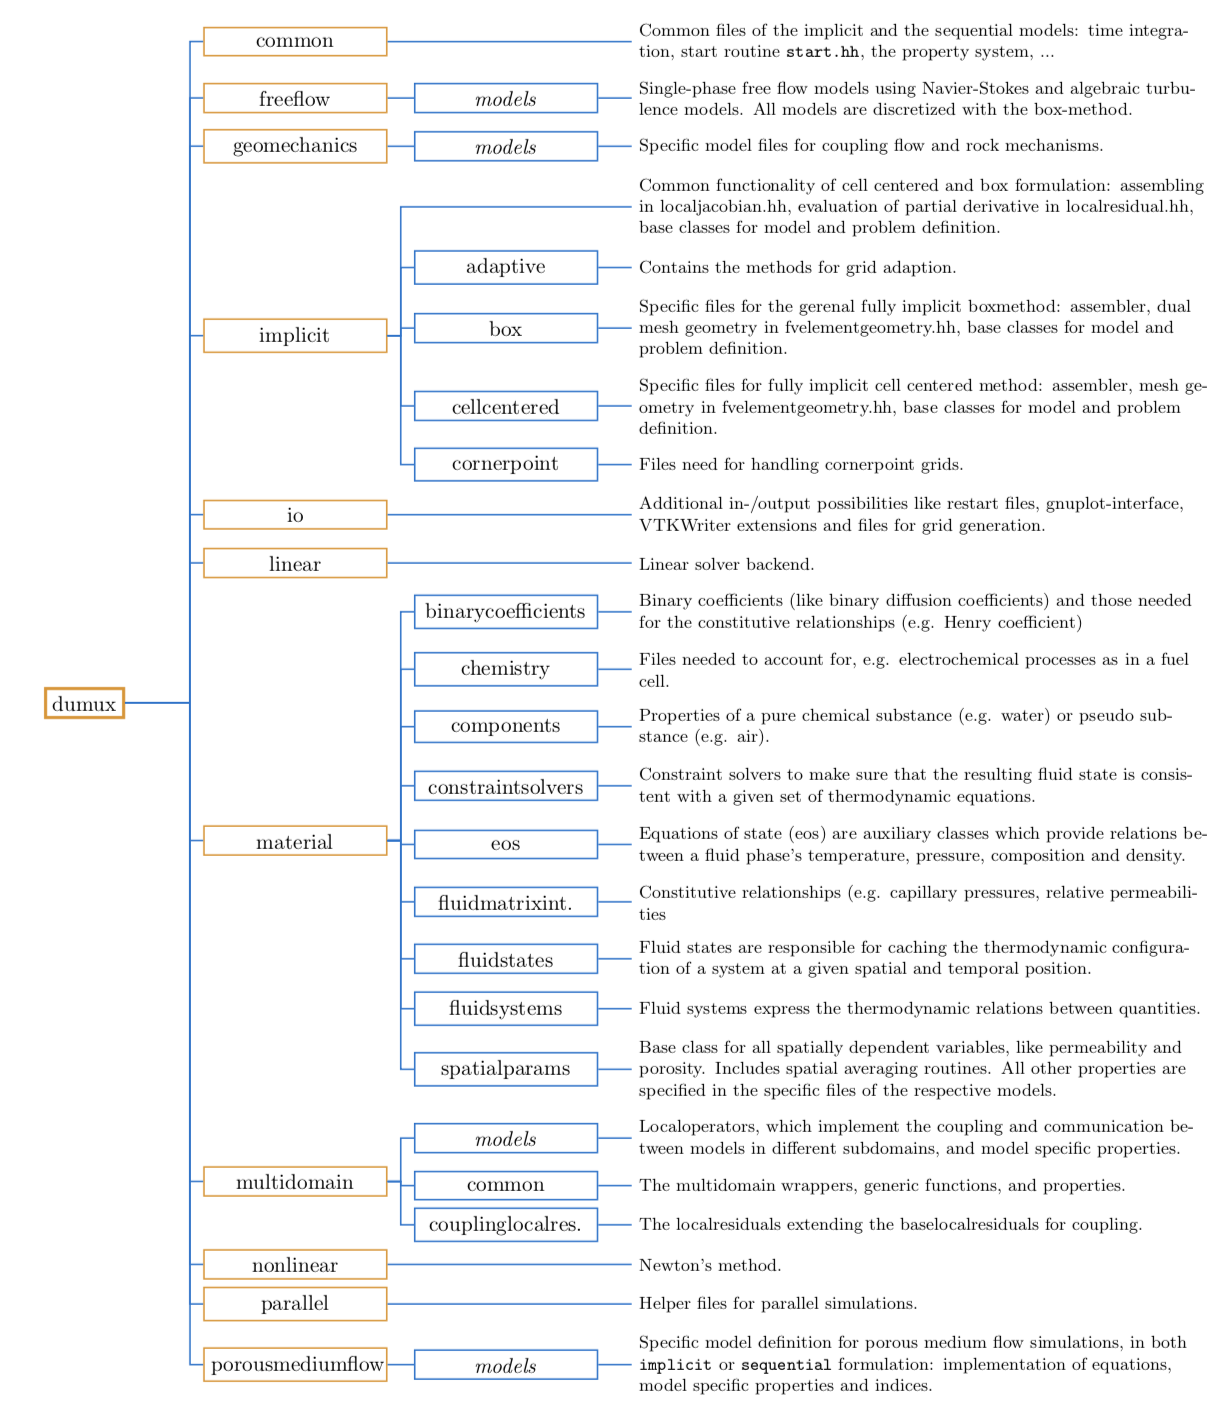
\includegraphics[height=190mm]{dumux_structure}
\caption{\footnotesize The $DuMu^x$ Structure}
\label{fig:dumux_structure}
\end{figure}\\\\

\newpage
\subsubsection*{Available Numerical Solvers}
%What solvers can we use ?
%What can DuMuX offer ?

$DuMu^x$ offers a large variety of numerical solvers that be implemented when defining the problem-file. This provides large flexibility in terms of computational cost and stability questions. \cite{flemischdumux}
\\One has to take care to choose a solver that is compatible with the given problem...

\subsubsection{Implemented Model}
%Explain Coupling of Tracer.

While $DuMu^x$ has a modular structure, some of the existing test cases can be combined to solve a more sophisticated and specific problem. In our case, this refers to the coupling of the existing tracer model to the 1p-1p model. While the 1p-1p model can simulate the flow of a solute in a network by convection and the diffusion of this solute into tissue, the tracer model can literally trace the path of this solute into the tissue, which can be used to obtain oxygen transport and diffusion into the tissue.

\subsubsection*{The 1p-1p Model}
%Briefly explain the 1p_1p Model
%Maybe put some results of the 1p_1p Model here

The 1p-1p model can compute pressure fields and velocities in vessel networks. The velocity outputs can then be used for the tracer model.

\subsubsection*{\footnotesize 1p-1p Model Impressions}

Figure \ref{fig:glom2_pressure}  is the result of a $DuMu^x$ blood flow simulation computed on a glomerulus network. The pressure field in the network is visualized.\\
\begin{figure}[h]
\centering{
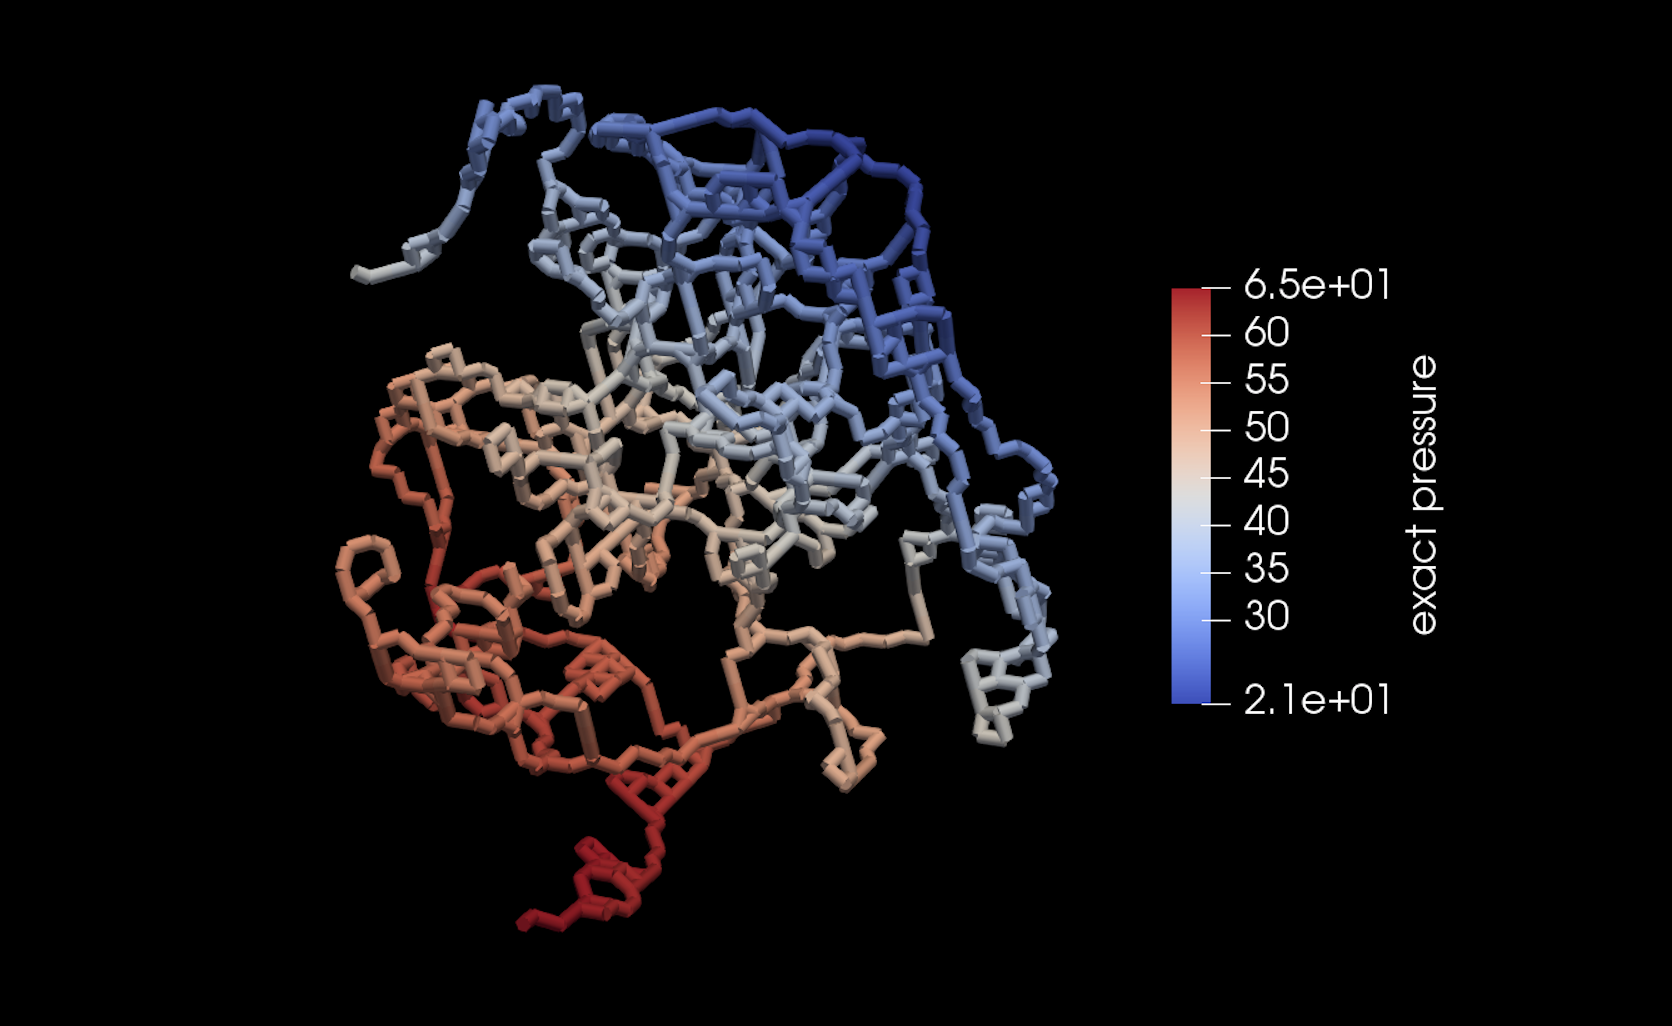
\includegraphics[width=162mm]{glom2_pressure}}
\caption{\footnotesize $DuMu^x$ Pressure Computations for Glomerulus Network}
\label{fig:glom2_pressure}
\end{figure}\\
%
\\Figure \ref{fig:glom2_velocity}  is the result of a $DuMu^x$ blood flow simulation computed on a glomerulus network. The velocity field in the network is visualized.\\
\begin{figure}[h]
\centering{
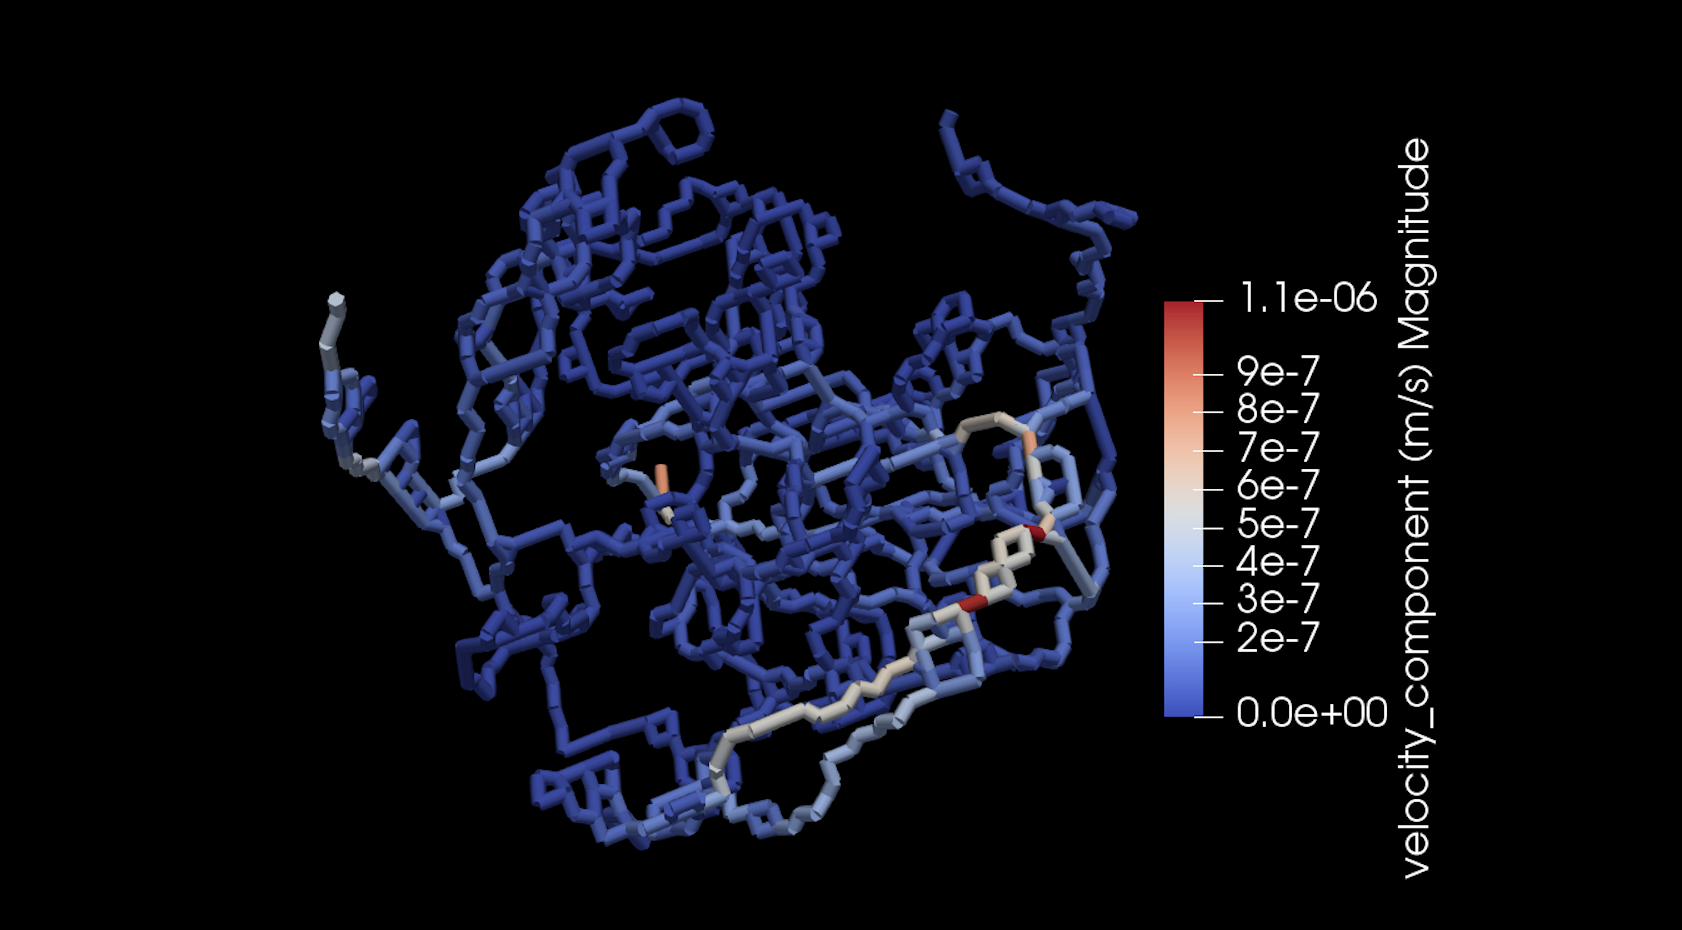
\includegraphics[width=162mm]{glom2_velocity}}
\caption{\footnotesize $DuMu^x$ Velocity Computations for Glomerulus Network}
\label{fig:glom2_velocity}
\end{figure}\\\\

\subsubsection*{The Tracer Model}
%Briefly explain the Tracer Model
%Maybe put some results of the Tracer Model here

The tracer model can trace substances in networks of different geometries, and accordingly compute concentrations and concentration fields of solutes in dynamic systems.\\
\\This is the reason I decided to choose the Tracer model to simulate the oxygen transport and diffusion in the given networks.\\
\\Generally, the tracer model is computing the distribution of a solute for every time step. It can either take velocities or flows as inputs, and gives the concentration of the traced solute as an output.
\\To briefly show what is meant by tracing a solute, a visualization for the first and last time of a tracing simulation is pictured in the following figures.\\
\\This simulation is a simple diffusion of Groundwater in a porous rock. The velocity field of the solute is assumed to be constant.

\subsubsection*{The Coupled Model}
%Briefly explain what coupling is and how code is supposed to work
%Hopefully put some results of the coupled model here or explain why the results are wrong

To achieve the goal of tracing oxygen in the given vessel-networks, I coupled the previously described models to obtain a 1p-1p-tracer model...
\\Using the velocity output of my previous 1p-1p model as an inpute for the tracer model, I wanted to get the concentration of my solute of interest, which is oxygen, for every time step.

\subsubsection{Input Data for the Simulations}
%Explain where the networks come from: CT by Willy and Artery/Vein recognition by Diego

The networks that were used for the simulations are extracted from real organs coming from mice. This process is done by scientists from different areas of expertise and is usually performed in the following order:
\\1)CT of the kidneys
\\2)Recognition of fat, tissue, arteries and veins by machine learning algorithms
\\3)Three dimensional captions of the organ are build by many virtual two dimensional slices
\\4)Transformation of the recognized artery/vein data into networks that can be used for the simulations.\\
\\The previously described tasks can be all be done by Interface Group members, which makes the working environment very special in terms independent research capabilities in this partially unchartered/unexplored field. %Can I say something like this or is it unnecessary/kind of bragging ?

%%%%%%%%%%%%%%%%%%%%%%%%%%%%%%%%%%%%%%%%%%%%%%%%%%
\newpage
\section{Simulation Results and Analysis}
%Put all the results here - Should be easier to understand things
In this section, the produced results using the two introduced methods will be presented and analyzed for a few different networks. Finally the results will be discussed and the methods will be compared.

\subsection{Results of the Green's Function Method}
%Main part of the Thesis
%Results part of Green's
%-Present some results on different networks
%- Plots and Results (maybe 3 I already have + 2 new ones)
%-Explanation of plots
%-Explaining inputs/outputs and meanings is in Appendix

The Green's Function Method is providing many outputs which are specified in more detail in the Appendix \ref{Outputs}. In this section, some of these outputs will be presented and explained. The physiological meaning will be described and finally the results will be discussed.

\subsubsection*{Krogh Model as an Introduction}
\label{Krogh}
%Explain relevance of this model and the produced results (many plots here)

%Present Network
The Krogh model describes the vessels as cylinders and the tissue as concentric cylinders surrounding the vessels. In this model, it is assumed that the capillaries are straight and parallel. The blood flow in all the capillaries is assumed to be unidirectional, and the distribution of capillaries is assumed to be homogeneous \cite{kreuzer1982oxygen}. As one might expect, this model has a few unrealistic assumptions, but as it is a straightforward network, it is the most basic model to start with to validate a computational method.\\
%Explain Plot
\\The Krogh model has been a standard simulation network used as an initial point for developments as it has a very easy and simple structure.
Figure \ref{fig:Contour_Krogh} is the result of a Green's Method blood flow simulation computed on a Krogh network. The Solute Concentration in the network and in the tissue is visualized in the form of a slice (see output section \ref{Outputs} for more information). The illustration shows an impression of oxygen levels in the tissue and the vessel segments, and generally gives the local oxygen concentrations in mmHg.\\\\
\begin{figure}[h]
\centering
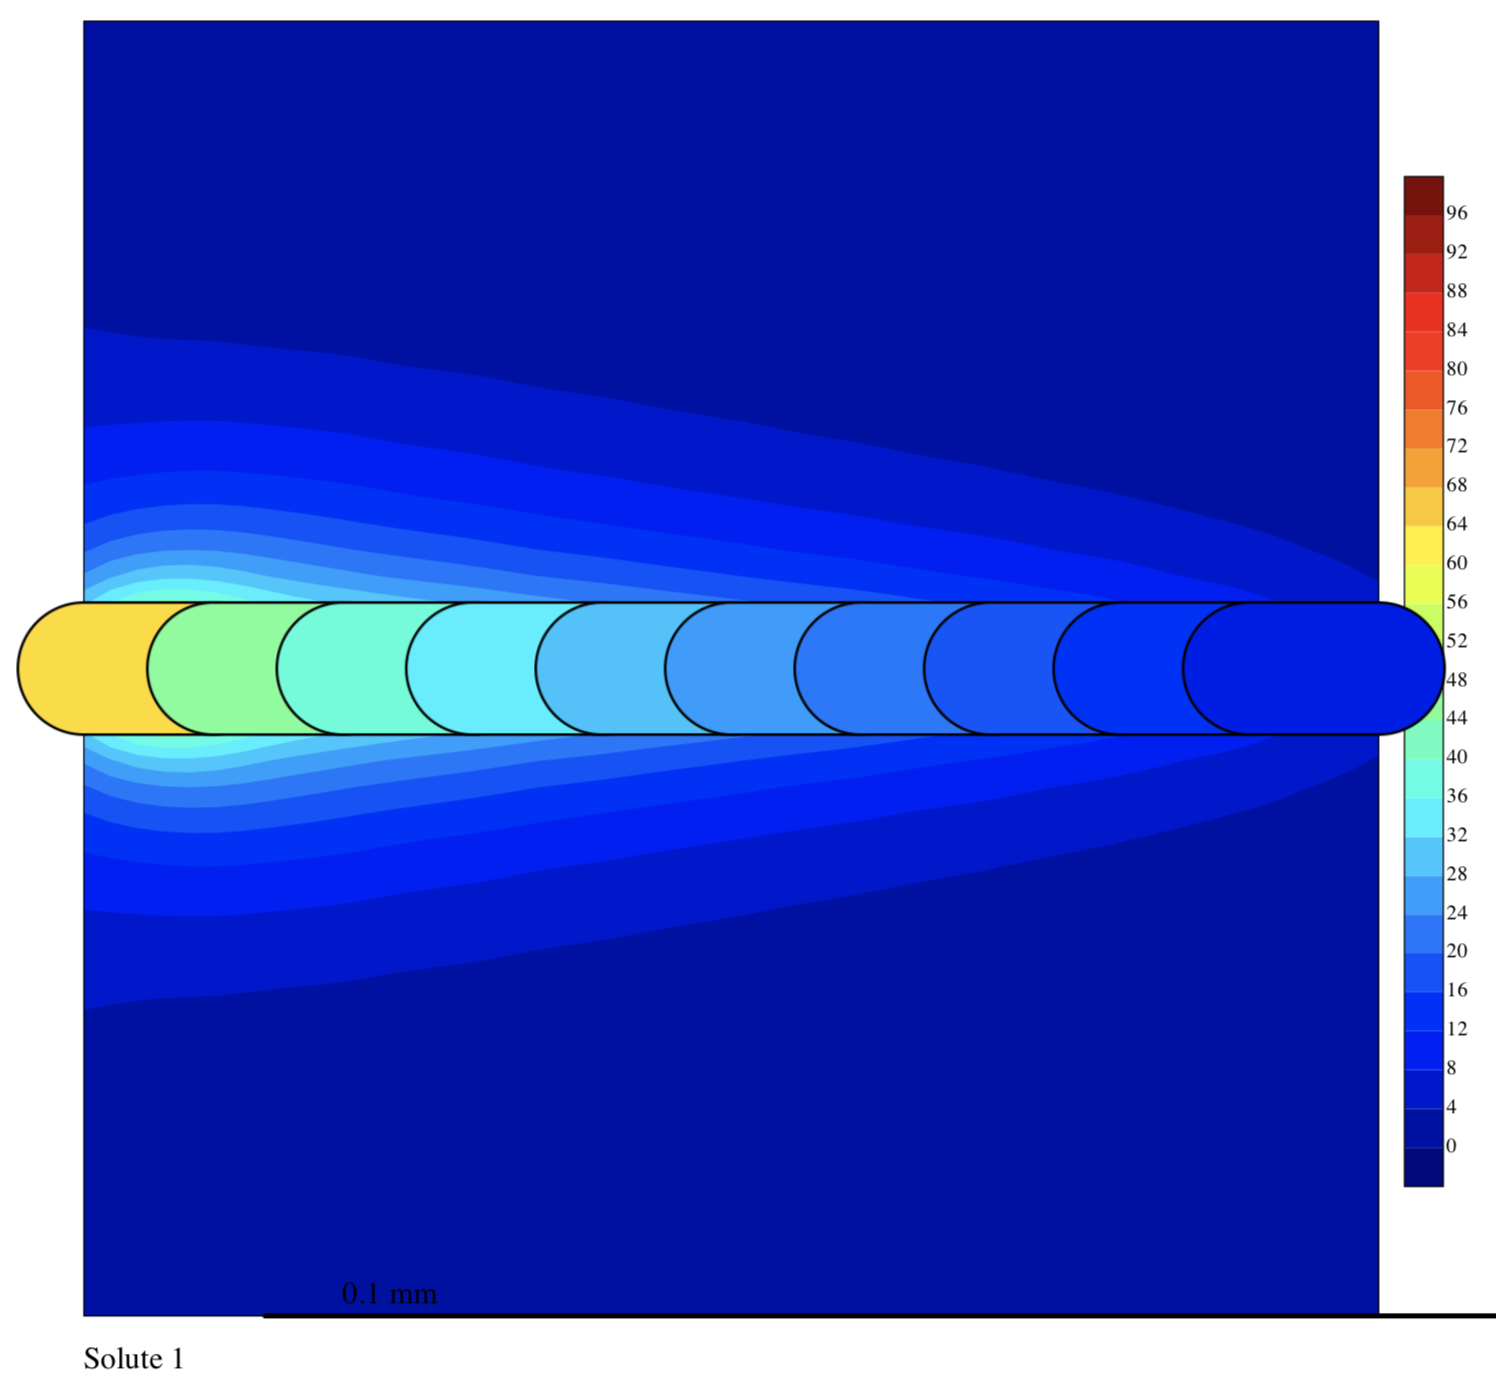
\includegraphics[width=120mm]{Contour_Krogh}
\caption{\footnotesize Green's Contour Output for Krogh Network}
\label{fig:Contour_Krogh}
\end{figure}
%Explain Results
\\One can clearly see that the results produced are physically realistic. On \ref{fig:Contour_Krogh} the blood flow goes from left to right. The $O_2$ concentration in mmHg accordingly goes down in flow direction. The concentrations as well as the diffusive distance in the tissue also decrease in flow direction, which can be explained by the fact that a lower concentration gradient goes with a lower diffusive flux. This is in accordance with Fick's Law of Diffusion \ref{Fick}. As one can see from the input files \ref{Inputs}, the diffusivity constant $\alpha$ is constant for homogeneous tissue. Due to the fact that the diameter of the vessels is constant as well when considering the Krogh model, the intravascular resistance to radial oxygen transport K for each diameter/vessel is also constant. Differences in diffusive fluxes and oxygen penetration distances into the tissue therefore mainly depend on the $PO_2$ gradients themselves.\\
\\Eventually, one can see that the results computed on the Krogh network show that the Green's function method performs well and produces physically accurate results on simplified and perfectly homogeneous networks as this one.
\\It is further remarked that analytical solutions of the Krogh cylinder model have been derived before and the results shown in this figure correspond well to the  analytical results. This validates that the Green's function method and the corresponding implementation can produce physically accurate results, and suggests that it is a suitable method to conduct further studies.

\newpage
\subsubsection*{A First Tumor Network}
%Explain relevance of this model and the produced results (many plots here)

%Present Network
The Green's function code provided by Prof. Secomb contains a few microvasculature networks as examples, which can be studied and extended. In this thesis, I executed many of those models to get a good understanding of physiological phenomena concerning $O_2$ transport in various organs and different networks.
\\Two of these example networks provided by Prof. Secomb are the tumor networks. I will first present the results obtained for the first network, and later get to the more complex and relevant second example.
\\The Tumor 1 network is more complicated than the previously presented Krogh model but generally gives a way better insight to the results than the Cardiac Network simulation, due to the much lower vessel density. The result is visualized on Figure \ref{fig:Contour_Tumor1998}. One can see the result of a Green's method blood flow simulation computed on a simple tumor network. As for the previous network, the oxygen concentration in the network and in the tissue is visualized in the form of a two dimensional slice (see output section \ref{Outputs} for more information). Again the illustration shows an impression of oxygen levels in the tissue and the vessel segments, and generally gives the local oxygen concentrations in mmHg.\\\\
%Explain Plot
The Tumor network provided by Secomb was used for further simulations and to validate the produced data.
Figure \ref{fig:Contour_Tumor1998}  is the result of a Green's method blood flow simulation computed on a tumor network. The solute concentration in the network is visualized.\\
\begin{figure}[h]
\centering
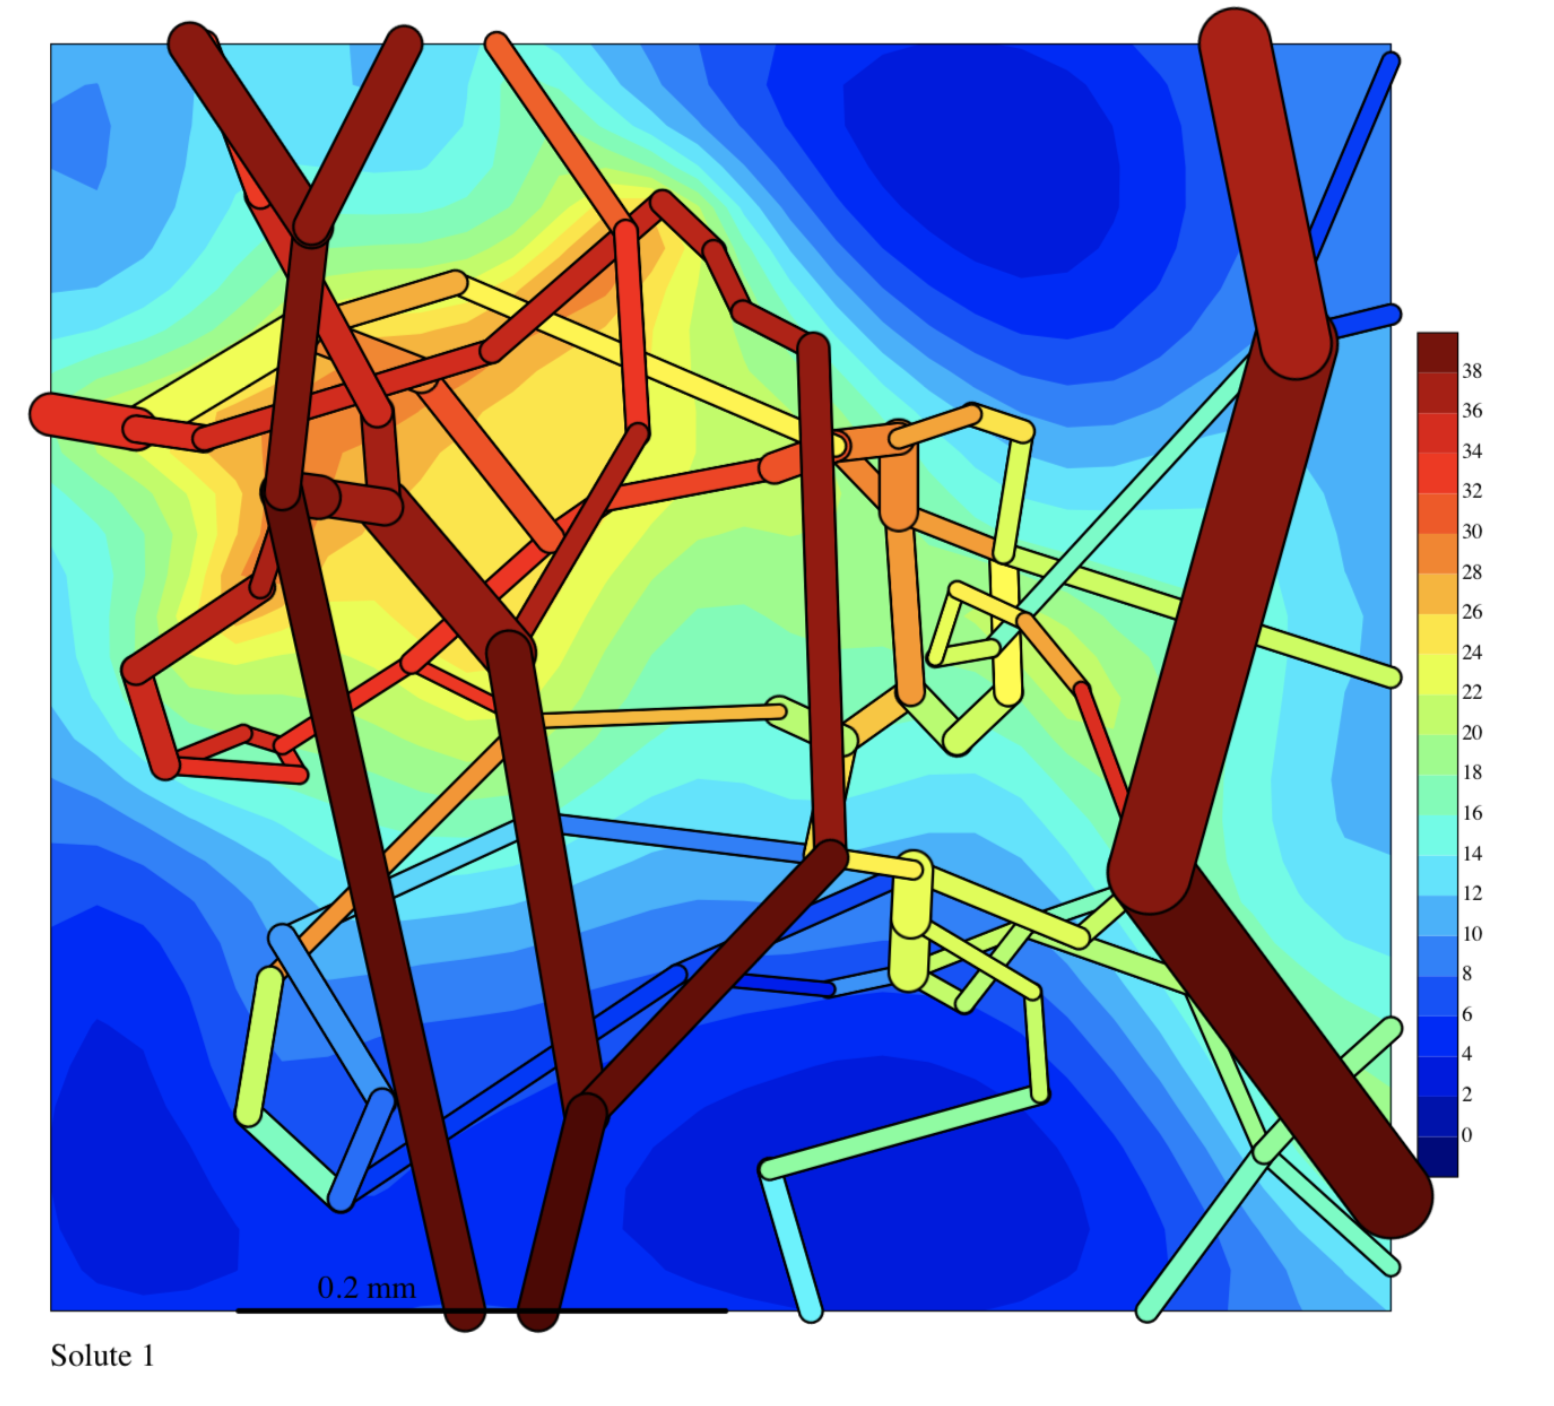
\includegraphics[width=120mm]{Contour_Tumor1998}
\caption{\footnotesize Green's Contour Output for Tumor 1}
\label{fig:Contour_Tumor1998}
\end{figure}\\
%Explain Results
\\As contour-plots generally show a \emph{compressed} picture of a three dimensional network, many vessels that are \emph{above} each other are shown as if they were intersecting. This can be hard to differentiate for the output files of some complex networks. In this case, this tumor network doesn't have many vessels, but is rather supplied by a few thicker vessels. The red color corresponds to oxygen enriched blood, and clearly oxygen in tissue regions proximal to these vessels is higher. There is no information given about the exact origin of this particular image segmentation and it can be observed that the length of segments within vessels is quite large. This is a limitation in order to obtain a precise resolution of the computed oxygen field, as $PO_2$ is always computed for each node and segment. Eventually a $PO_2$ value is assigned to each segment. This means that a lower resolution for the oxygen field is obtained.
\\In this case, $PO_2$ levels reach up to about $40$ mmHg which lies within the physiological range.

%\subsubsection*{Brain Model}
%Explain relevance of this model and the produced results (many plots here)

%The Brain network provided by Secomb (?) was used for further simulations and to validate the produced data.

\newpage
\subsubsection*{The Cardiac Network}
%Explain relevance of this model and the produced results (many plots here)
%The Cardiac network provided by Secomb was used for further simulations and to analyze results in more complex networks.\\

%Present Network
Another interesting example network is the cardiac network. Even though there is no information given about how this particular image segmentation was obtained, knowing that it is a cardiac network, one might expect a high density of vessels for this network.
\\In this section, the oxygen distribution in a cardiac network will be presented. This network is more complicated than the previously presented Krogh model \ref{Krogh}. The result is visualized on Figure~\ref{fig:Contour_Cardiac1}. The given output shows the result of a Green's method blood flow simulation computed on a cardiac network. As for the Krogh model, the oxygen concentration in the network and in the tissue is visualized in the form of a slice (see output section \ref{Outputs} for more information). Again the illustration shows an impression of oxygen levels in the tissue and the vessel segments, and generally gives the local oxygen concentrations in mmHg.\\
%Explain Plot
\begin{figure}[h]
\centering
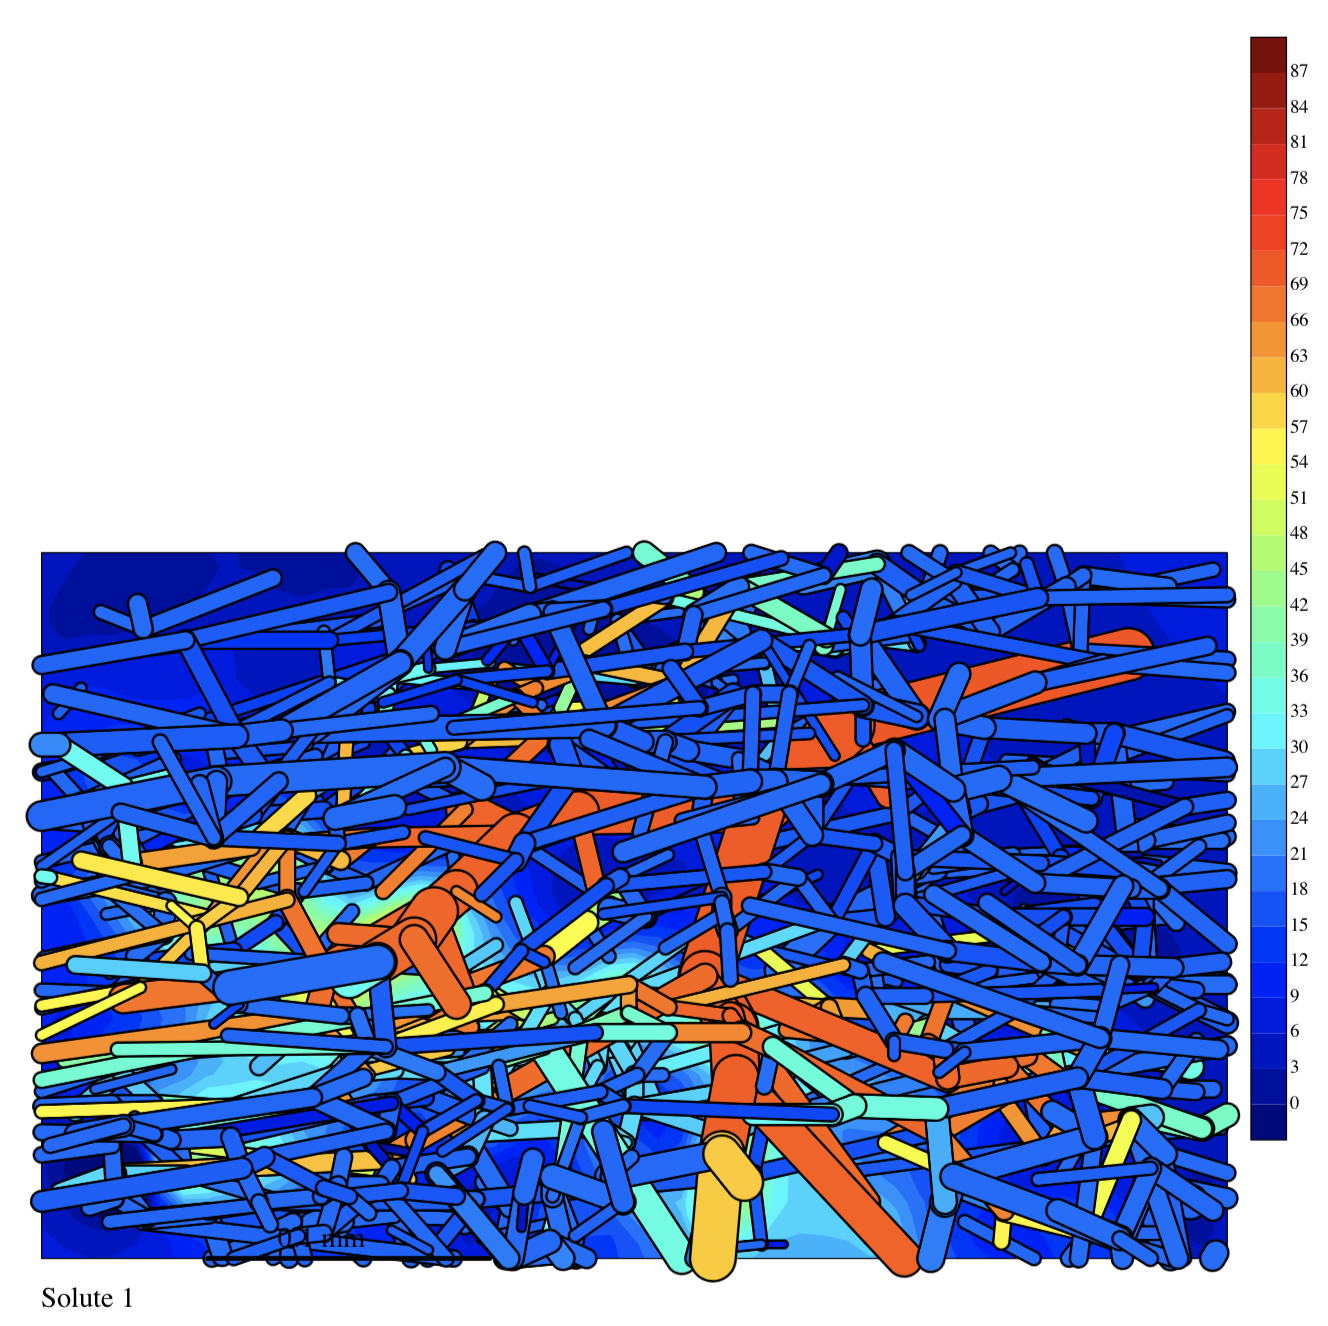
\includegraphics[width=120mm]{Contour_Cardiac}
\caption{\footnotesize Green's Contour Output for Cardiac Network}
\label{fig:Contour_Cardiac1}
\end{figure}
\\Figure~\ref{fig:Contour_Cardiac1} shows the distribution of Oxygen in a small
network of vessels.
%Explain Results
\\The three dimensional network of vessels is \emph{compressed} to a two
dimensional representation in order to get a simpler output file. This kind of output has the advantage of encapsulating most of the computed values, even though it might look complex for some networks where the oxygen fields are very heterogeneous. The red color corresponds to oxygen enriched blood. The principle vessels go through the middle of the three dimensional tissue section and therefore have the highest oxygen partial pressures which are around $65$ mmHg. The oxygen concentration in the finer and smaller vessels surrounding the big oxygen-supplying vessels accordingly decreases with growing distance from the oxygen sources. {\color{red}For this contour-plot, it is hard to extract a lot of information about the tissue concentrations, as mostly the vessels are pictured due to the complexity of the network. Is this phrase okay Kartik ?}
But still the oxygen in tissue regions proximal to the bigger oxygen-supplying vessels is higher. Once again, it can be observed that the length of segments within vessels is quite large, which causes a lower oxygen field resolution.
\\The $PO_2$ levels reach up to about $84$ mmHg within a physiological range.

\newpage
\subsubsection*{The Mesenteric Artery Network}
%Explain relevance of this model and the produced results (many plots here)
%The Mesenteric Artery network provided by Secomb was used for further simulations and to get more computational results.\\

%Present Network
Another example network provided by Prof. Secomb is the mesenteric artery network.
\\Like for the previously presented networks, there is no information given about how this particular image segmentation was obtained and where it comes from. Knowing that this network is supposed to represent a mesenteric artery network, which is an artery supplying the large intestine, one can clearly see the very small vessels surrounding the main arterial tree. These vessels are embedded in the intestine itself and supply oxygen to the surrounding cells.
\\Generally the vessels are very fine and the vessel resolution is high, which entails a good oxygen field resolution for the tissue surrounding the vessels.
\\The result is visualized on Figure \ref{fig:Contour_Mesent1}. The output shows the result of a Green's method blood flow simulation computed on a mesenteric artery network. As for the previous networks, the oxygen concentration in the network and in the tissue is visualized in the form of a slice (see output section \ref{Outputs} for more information). Again the illustration shows an impression of oxygen levels in the tissue and the vessel segments, and generally gives the local oxygen concentrations in mmHg.
%Explain Plot
\begin{figure}[h]
\centering
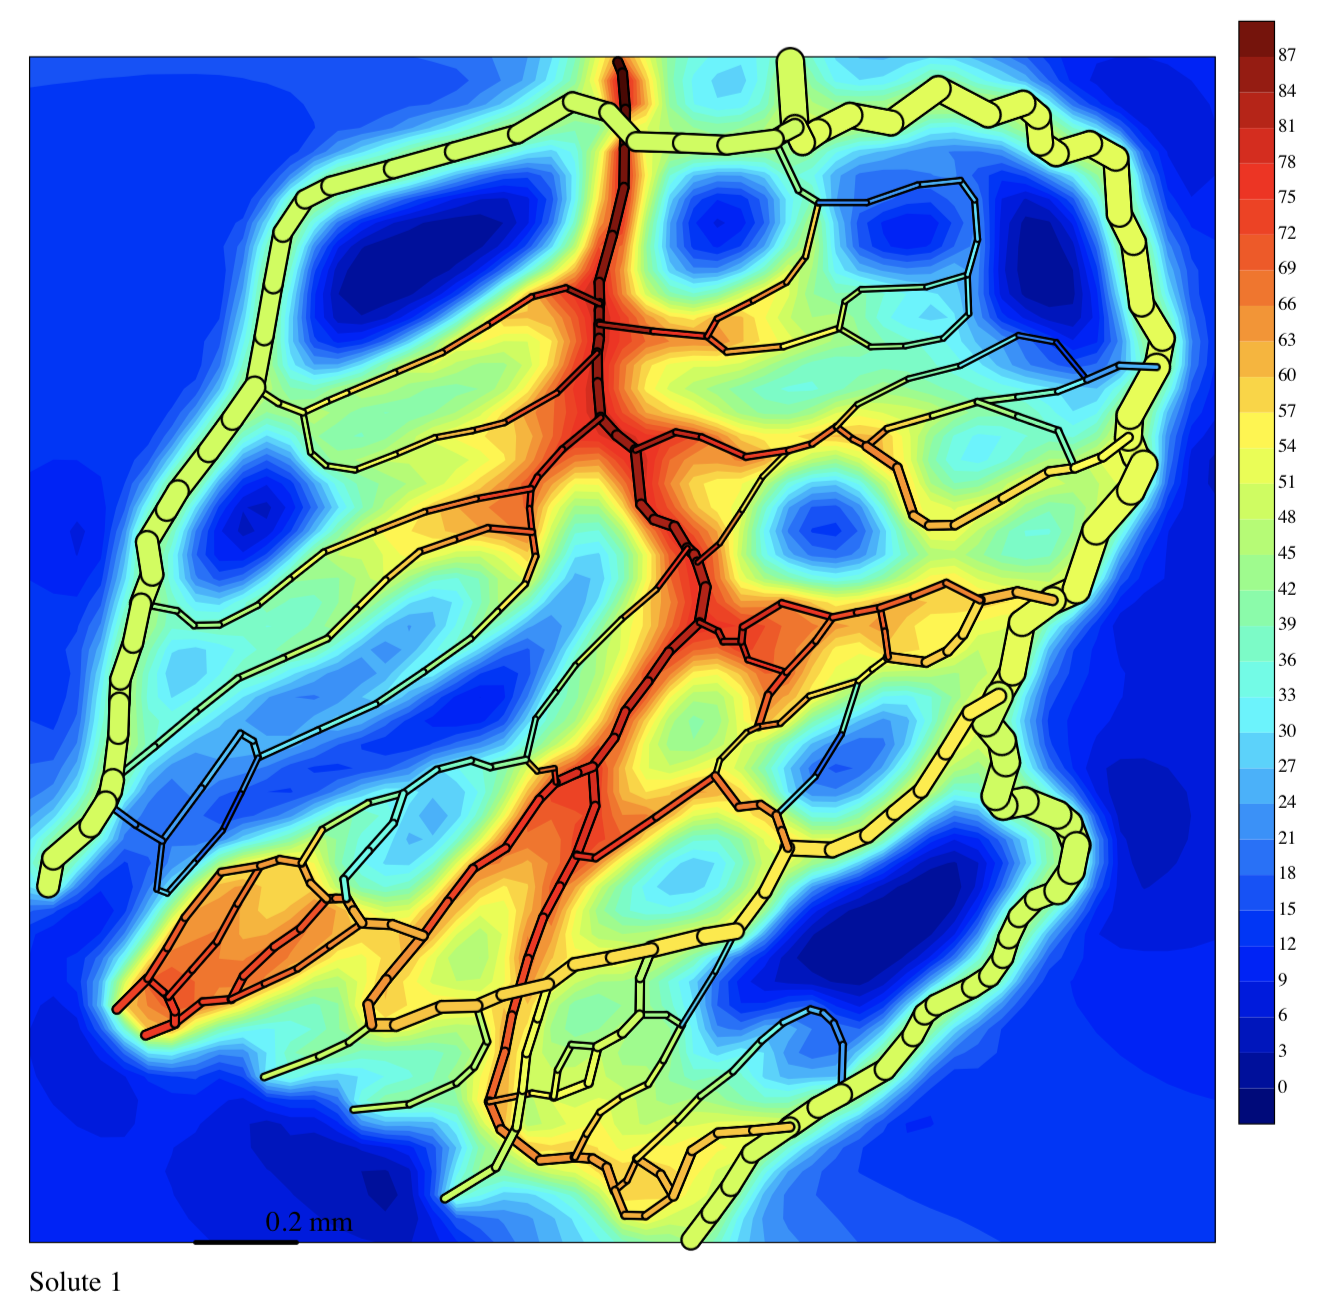
\includegraphics[width=120mm]{Contour_Mesent1}
\caption{\footnotesize Green's Contour Output for a Mesenteric Artery Network (Solute 1)}
\label{fig:Contour_Mesent1}
\end{figure}
%
%\\Figure \ref{fig:Contour_Mesent2}  is the result of a Green's Method blood flow simulation computed on a Mesenteric Artery network. The Solute Concentration of Solute 2 in the network is visualized.\\
%\begin{figure}[h]
%\centering
%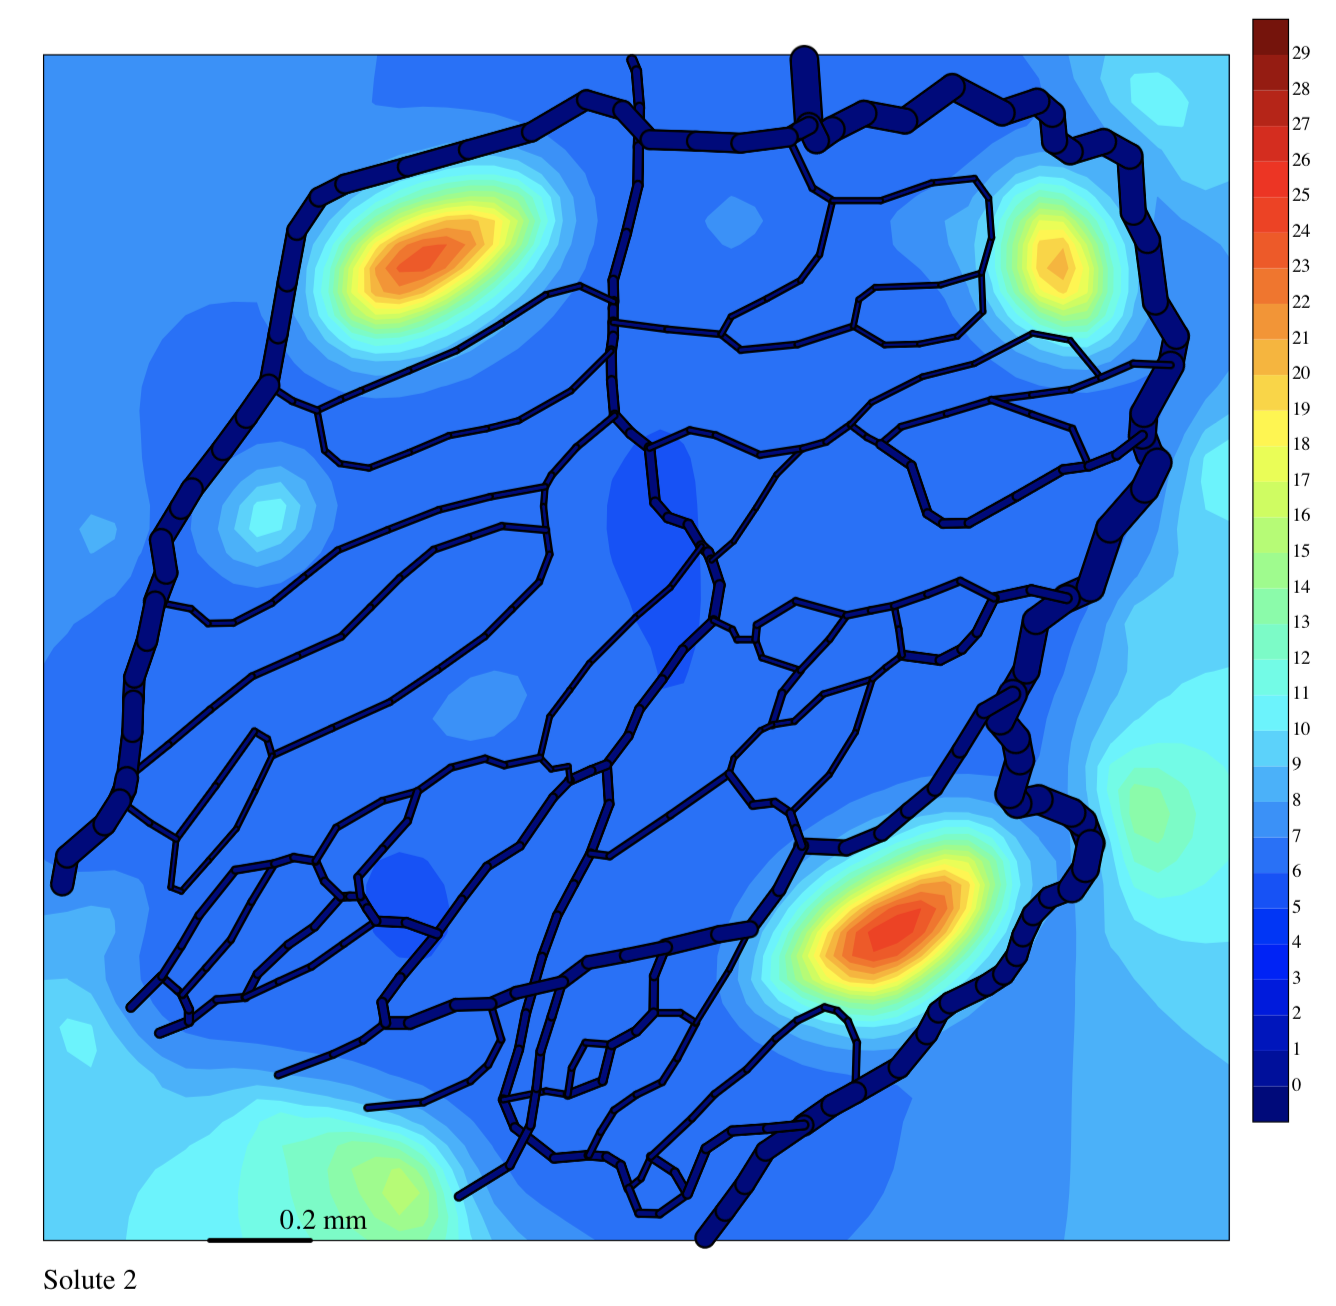
\includegraphics[width=85mm]{Contour_Mesent2}
%\caption{\footnotesize Green's Contour Output for a Mesenteric Artery Network (Solute 2)}
%\label{fig:Contour_Mesent2}
%\end{figure}
\\
%Explain Results
\\This network is more complicated than the previously presented networks but generally gives a better insight to the results than the cardiac network simulation, due to the much lower vessel density {\color{red} are you okay with this ? do you think that this gives a better insight or should I remove this sentence ?}. Especially the tissue concentrations and the changing oxygen concentrations in longitudinal direction of the vessels can be seen very well.
\\Due to the low density of capillaries for this network, this figure can give a good insight to the values computed by the Green's Model. One can clearly see that the partial pressure of $O_2$ goes down in radial direction with growing distance from the vessels. At hotspots where the capillary density is higher due to branching and ramification, the diffusion comes from two vessels and the superposition of two close source elements leads to peaks in $PO_2$ values.\\
\\From a physiological point of view, the computational result is correct when assuming that the oxygen consumption through the whole intestine is constant. The oxygen supply to the intestinal vessels surrounding the main arterial tree is constant, and the oxygen concentrations in the intestinal ares are slightly above 50 mmHg, which is in the physiological range.
\\The general oxygen field clearly shows that some hypoxic regions can be found at spots without vessel or where the vessels themselves have a very low $PO_2$ concentration. With $PO_2$ values ranging from $0$ mmHg (hypoxic region) to 87 mmHg, the results for the whole sample lie once more in the physiological range.
\\{\color{red} what do you think about the qualitative discussion on physiological level ? I read a few things about the mesenteric artery and thought this might be interesting, but wanted to ask you what you think.}

\newpage
\subsubsection*{A Second Tumor Network}
%Explain relevance of this model and the produced results (many plots here)

%Present Network
Another interesting tumor example network provided by Prof. Secomb is the Tumor 2 network.
\\Even though there is no information given about how this particular image segmentation was obtained, knowing that it is a tumor network, one might expect a random ramification and distribution of vessels. In fact, this network is build by vessels of different sizes and the oxygen concentrations within the vessels is largely varying.
\\The Tumor 2 network is more complicated than the previously presented Tumor 1 network and the computational simulation produces a very interesting output. The result is visualized on Figure \ref{fig:Contour_TumorDuke}. Here one can see the result of a Green's Method blood flow simulation computed on a simple Tumor network. As for the previous models, the Oxygen Concentration in the network and in the tissue is visualized in the form of a slice (see output section \ref{Outputs} for more information). Again the illustration shows a virtual cut into the tissue and gives local oxygen concentrations in mmHg.\\\\
%Explain Plot
Figure \ref{fig:Contour_TumorDuke}  is the result of a Green's method blood flow simulation computed on a tumor network. The oxygen concentration in the network and the tissue is visualized.\\
\begin{figure}[h]
\centering
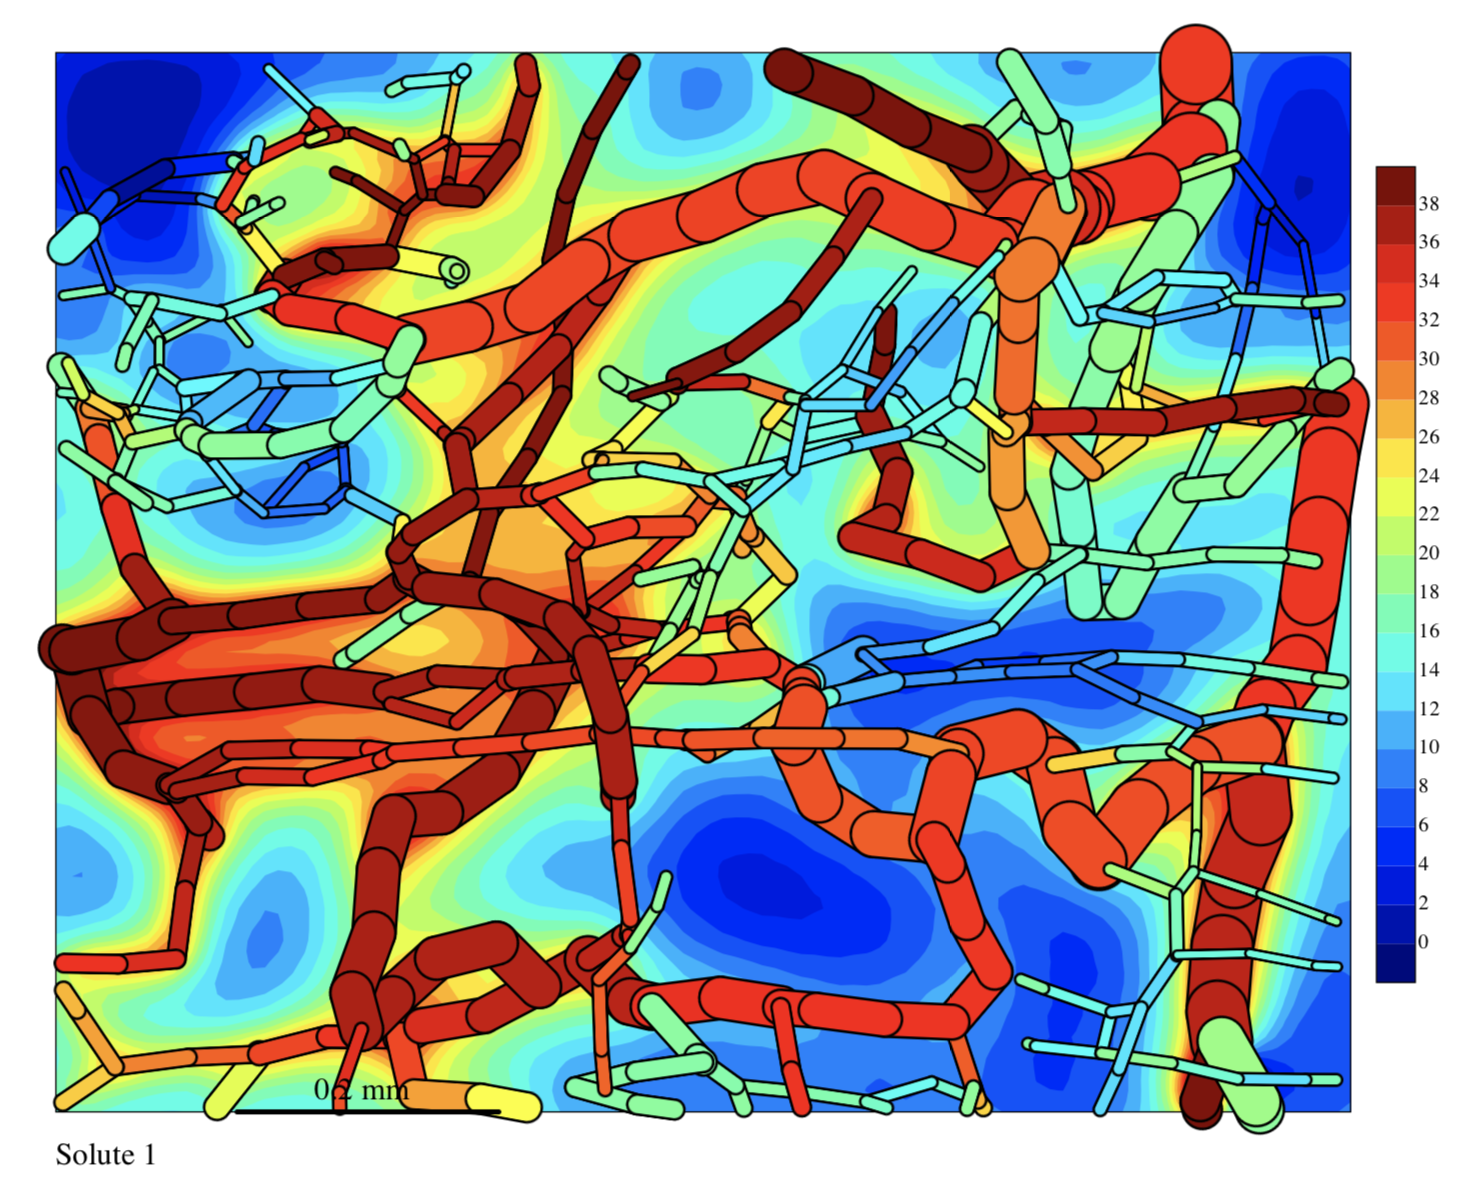
\includegraphics[width=120mm]{Contour_TumorDuke}
\caption{\footnotesize Green's Contour Output for Tumor 2}
\label{fig:Contour_TumorDuke}
\end{figure}\\
%Explain Results
\\The overlapping of the vessels with different oxygen concetrations is due to the fact that three the dimensional network of vessels is \emph{compressed} as for the previous examples. The red color corresponds to oxygen enriched blood which is in this case carried by the thicker vessels supplying this sample of tissue. The oxygen partial pressure in the tissue regions proximal to these bigger vessels is higher with peaks around $40$ mmHg. The segmentation resolution depends on the vessel, but is overall rather high, which induces/entails {\color{red} (which expression is better ?)} a high resolution for the oxygen field in the tissue.
\\Generally the highest $PO_2$ levels can be found surrounding the big vessels and especially in regions where many sources are overlapping. This is due to the fact that the source terms are superpositioned when calculating the oxygen field during the computational iterations, and makes sense from a physiological point of view, as a lot of oxygen is supplied to these areas.
\\The $PO_2$ levels range between around $3$ and $40$ mmHg within a physiological range. Generally the average $PO_2$ in this sample is quite high, due to the equally distributed and well oxygenated big vessels.

\newpage
\subsubsection*{Further Outlook for New Networks}
%Explain relevance of the new models and the produced results (many plots here)
%These results are wrong !!! why ?
%In this section the goal is to see how this method can perform in general when it is applied to new networks and to discuss the produced results in detail.

An overview to simulation results of the Green's method were presented for different networks, covering a range from homogeneous and simple network to rather complex, heterogeneous and physiologically interesting samples.
\\Considering how well this method seems to perform for some complex networks I presented in the last section, I asked myself how well this method can perform for networks. For this reason I used did the simulation on a glomerulus network, which I already used for $DuMu^x$ simulations {\color{red} what do you think about this formulation ?}.
\\Even though oxygen computations with diffusion into the tissue is physiologically meaningless for a glomerular network {\color{red} you asked me not to use words like no sense, but I think it's okay in this case?}, as glomeruli are not surrounding by normal tissue, I only used the glomerulus as basic network, as if the network was embedded anywhere else in homogeneous tissue.
\\Figure \ref{fig:NetNodesSegs_Glom}  is the result of a Green's Method blood flow simulation computed on a glomerulus network. The Solute Concentration in the network is visualized.\\
\begin{figure}[h]
\centering
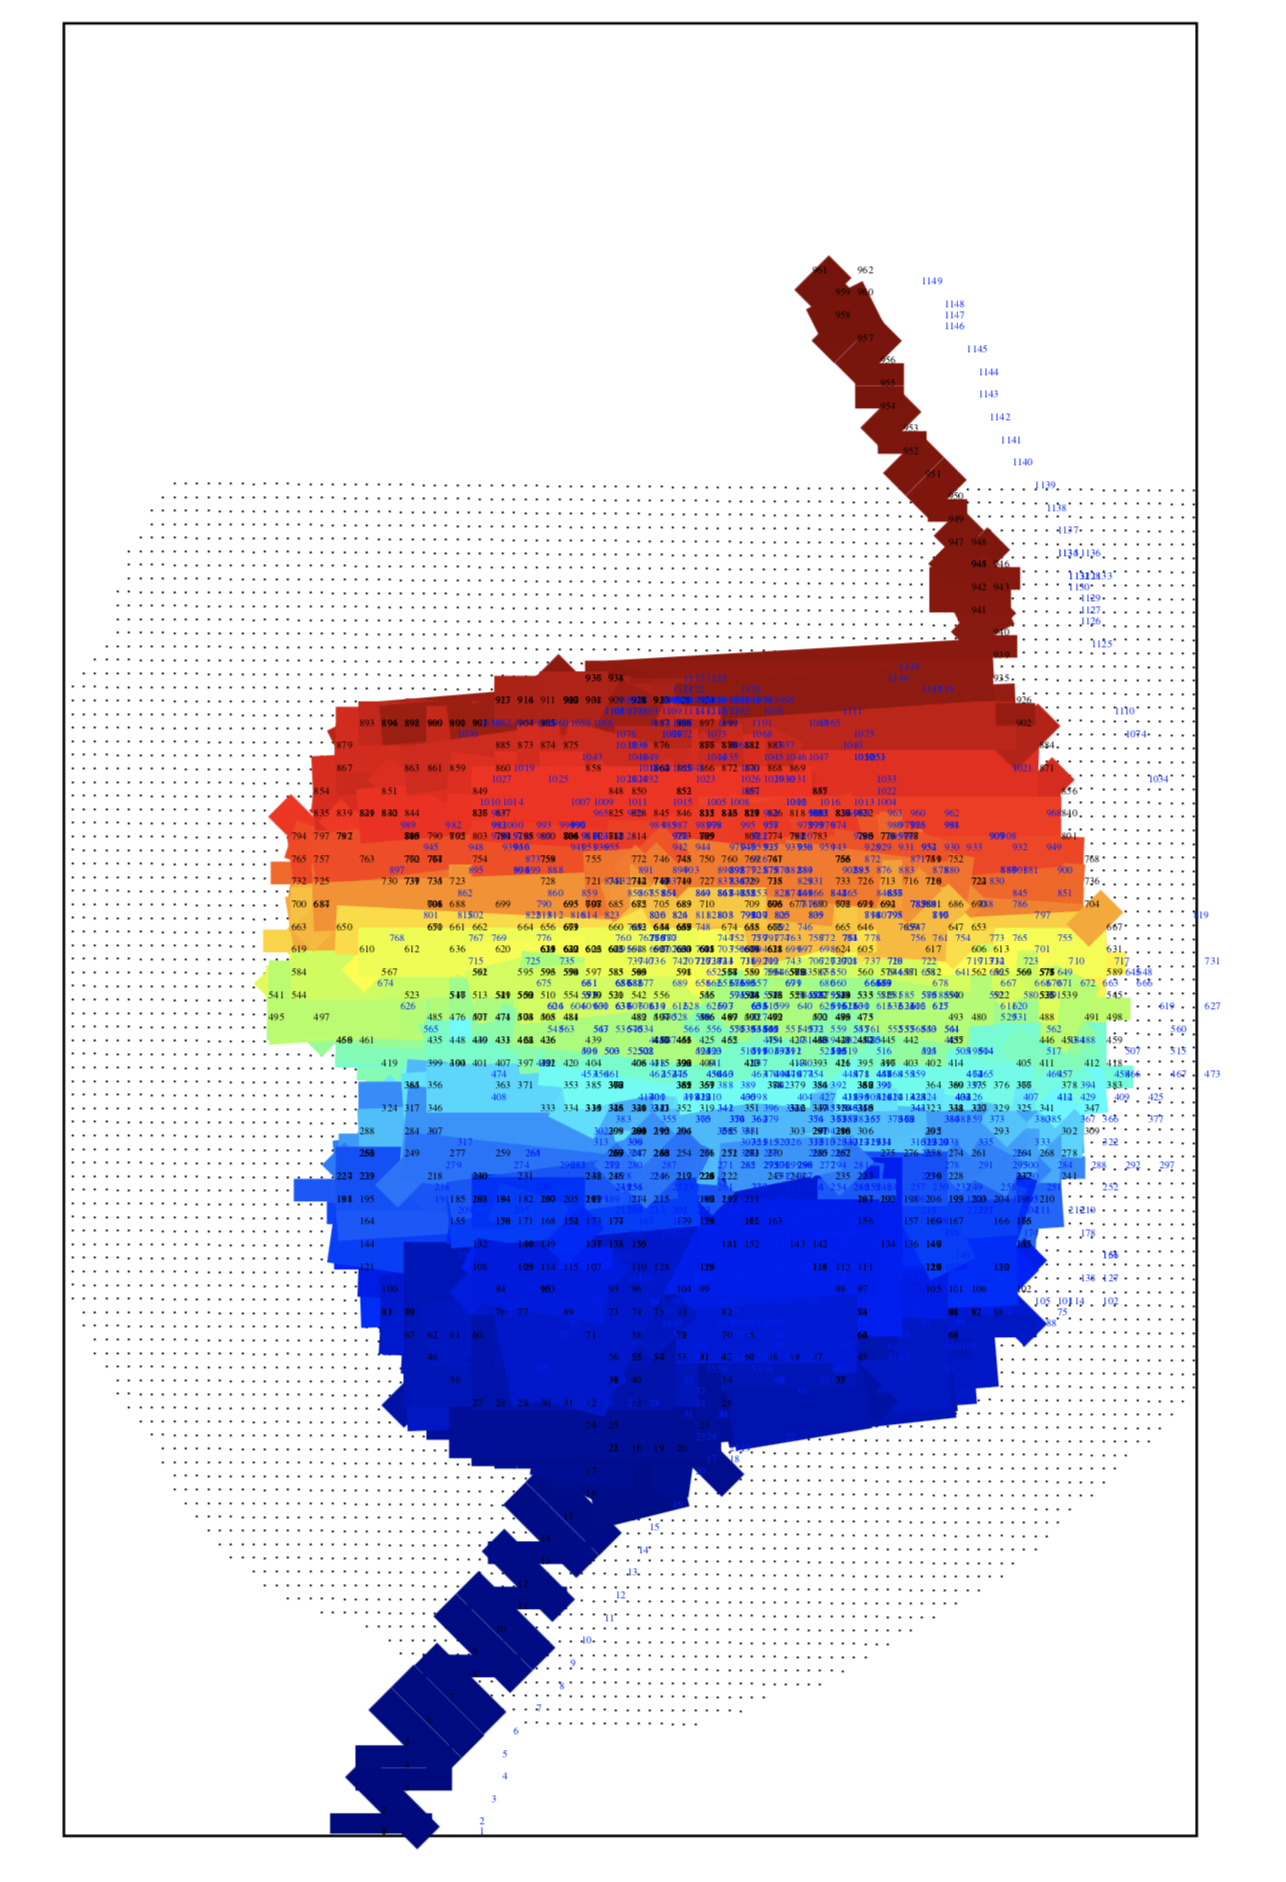
\includegraphics[width=100mm]{NetNodesSegs_Glom}
\caption{\footnotesize Green's Net Nodes Output for a Glomerulus Network}
\label{fig:NetNodesSegs_Glom}
\end{figure}
\\In this case the presented output file is not a contour plot, but rather a plot illustrating the computed oxygen levels in each node and vessel segment. This type of plot is called \emph{NedNodesSegs} and is supposed to give the computed oxygen partial pressure in mmHg for each segment and for each node.
\\In this part I would to mention that the code did not run as expected, and thus didn't produce a sink field. As the Green's method iteratively computes a source and a sink field, which are used to obtain the oxygen distribution field by superposition, no oxygen field could be computed. The numbers written on the output file \ref{fig:NetNodesSegs_Glom} are the numerations of the segments and the nodes (see output section \ref{Outputs} for more information).
\\This network could thus be segmented, but no computations in terms of oxygen field could be made, neither in vessels, nor in the virtual tissue - real glomeruli are not surrounded by tissue. The reasons for this failing are not clear, as the network is so complex, that no correct explanation can be given without doubts. There might also be a problem with the chosen parameters concerning the solute or the intravascular resistance (see Input Section \ref{Inputs} for more information).

\newpage
\subsection{Discussion of the Green's Method and the Produced Results}
%Discussion part of Green's
%Final thoughts about Green's Method for physiological applications and oxygen delivery simulations/computations.
%Compare the results with physiological measured values and check if the results make sense in general.

As the presented examples show, the Green's method and its implementation can produce some excellent results in terms of physical oxygen field simulations in networks.
\\The results are in accord with the previously described physical laws, which describe the oxygen transport from the vessel to the tissue. Moreover, the results are physiologically accurate. The computed values generally range between $0$ mmHg (hypoxic tissue) and $87$ mmHg (very well oxygenated tissue) and seem to be in the physiological range.
\\Even though these computations have been made on networks that were derived from real organic networks, no information was given about how the particular image segmentations were obtained. This also makes it hard to compare the results with real world values {\color{red} or how should I call this ? experimental values? another important question I might have is: do we have know if these network come from organs coming from mice/rats or whatever? as we don't know this, I would especially point out that the computed values cannot be compared to any specific values that we could expect or was measured in the past. we can only say that the values are in the physiological range and that the physical properties of oxygen transport and diffusion are well respected and in accord with the simulation results}, as we don't know anything in particular about the provenance of the networks.


\subsection{Results of $DuMu^x$} 
%Interesting but shorter part, due to the fact that DuMuX is not really producing anything yet
%Results part of DuMuX
%-Pros/Cons
%\\-Quality of results
%\\-Paraview Visualization of results

Using $DuMu^x$ \ref{$DuMu^x$} some blood flow simulations were run to evaluate the quality of results that can be produced using this software. This section will present and explain some results produced by $DuMu^x$, and some rather physical than physiological interpretations of simulation results will be discussed.

\subsubsection*{Some Glomerulus Network Simulations}
%I will hopefully put 1p_1p_tracer results here later
%Discuss the pressure drop from afferescent to effeverescent (?) vessel/artery
%Explain some physical things behind it and be creative

\begin{figure}[h]
\centering
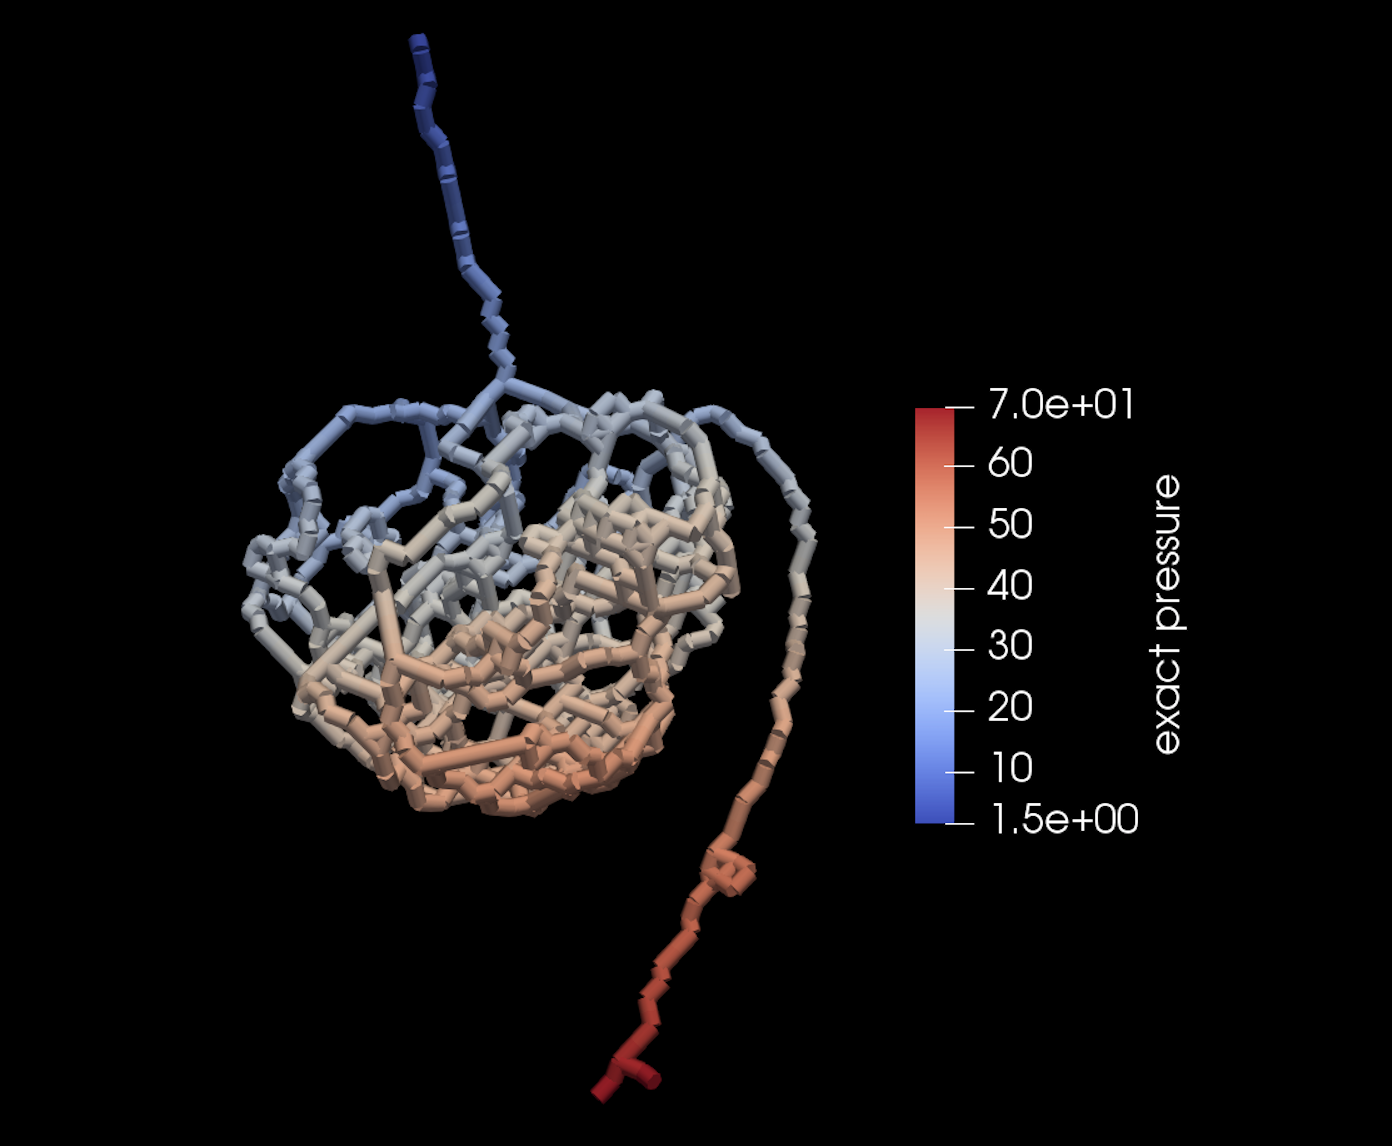
\includegraphics[width=162mm]{glom_pressure}
\caption{Pressure Field in Glomerulus 1}
\label{fig:glom_pressure}
\end{figure}
The figure \ref{fig:glom_pressure} is the result of a DuMuX 1p-1p blood flow simulation computed on a glomerulus network. The pressure field of the flow is visualized.\\

\begin{figure}[h]
\centering
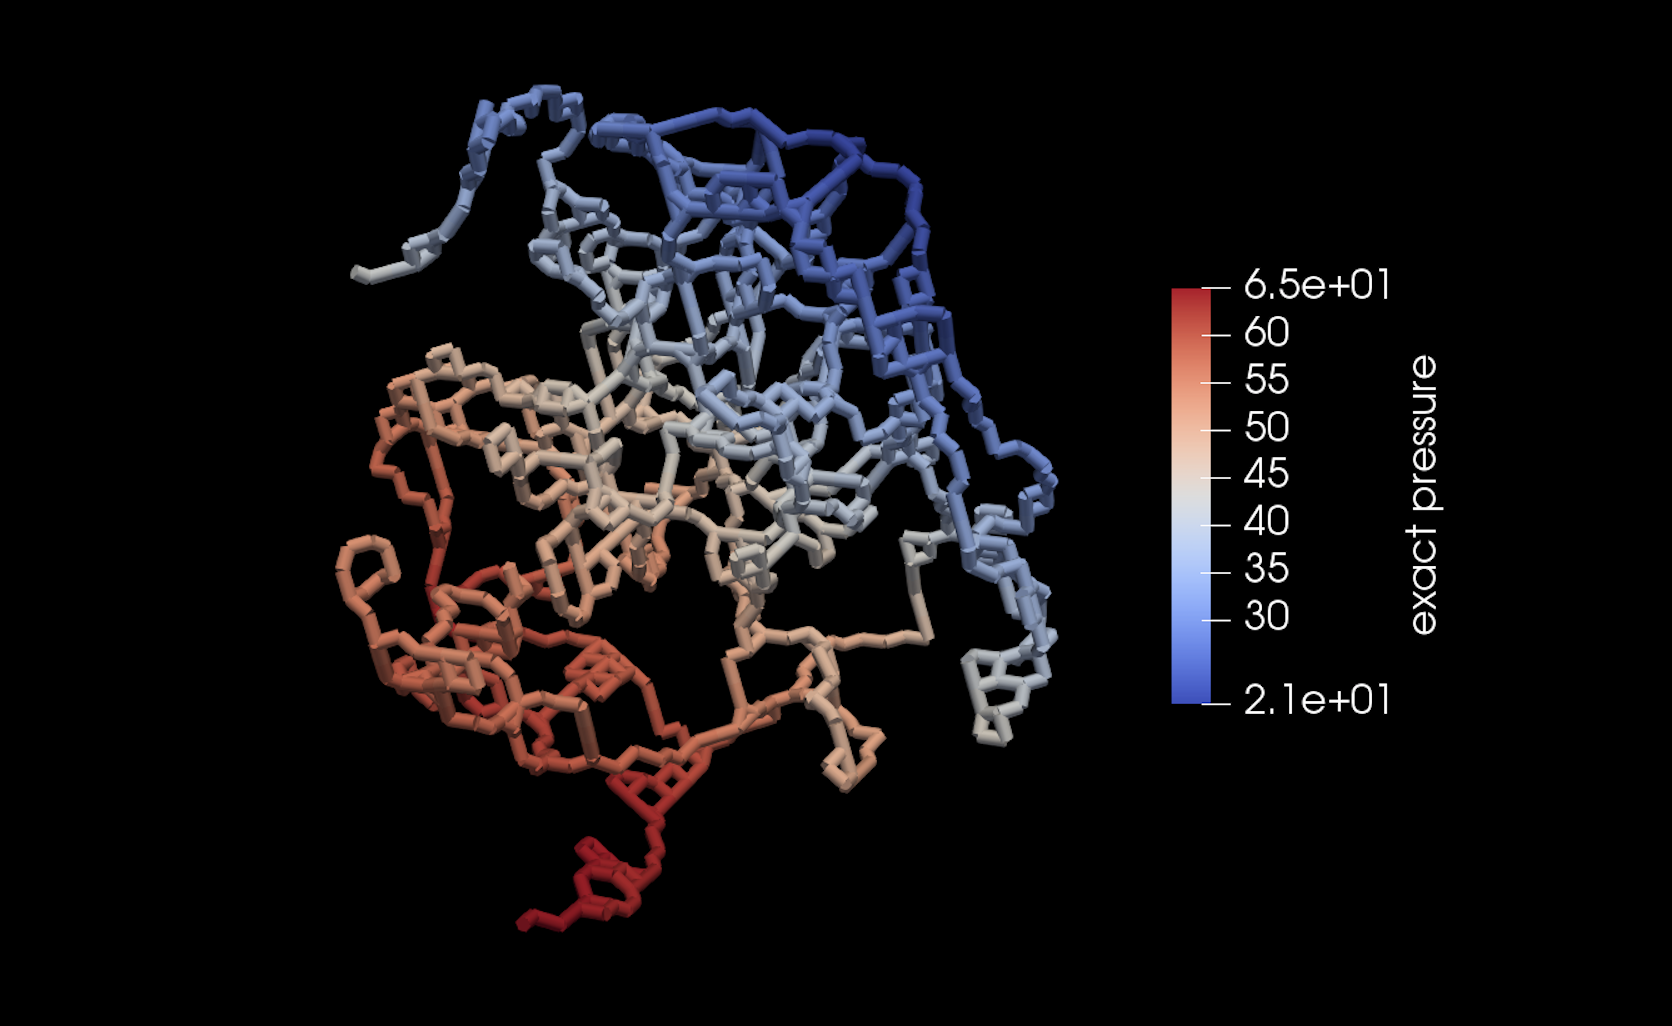
\includegraphics[width=162mm]{glom2_pressure}
\caption{Pressure Field in Glomerulus 2}
\label{fig:glom2_pressure}
\end{figure}
The figure \ref{fig:glom2_pressure} is the result of a DuMuX 1p-1p blood flow simulation computed on a Glomerulus network. The pressure field of the flow is visualized.\\

\begin{figure}[h]
\centering
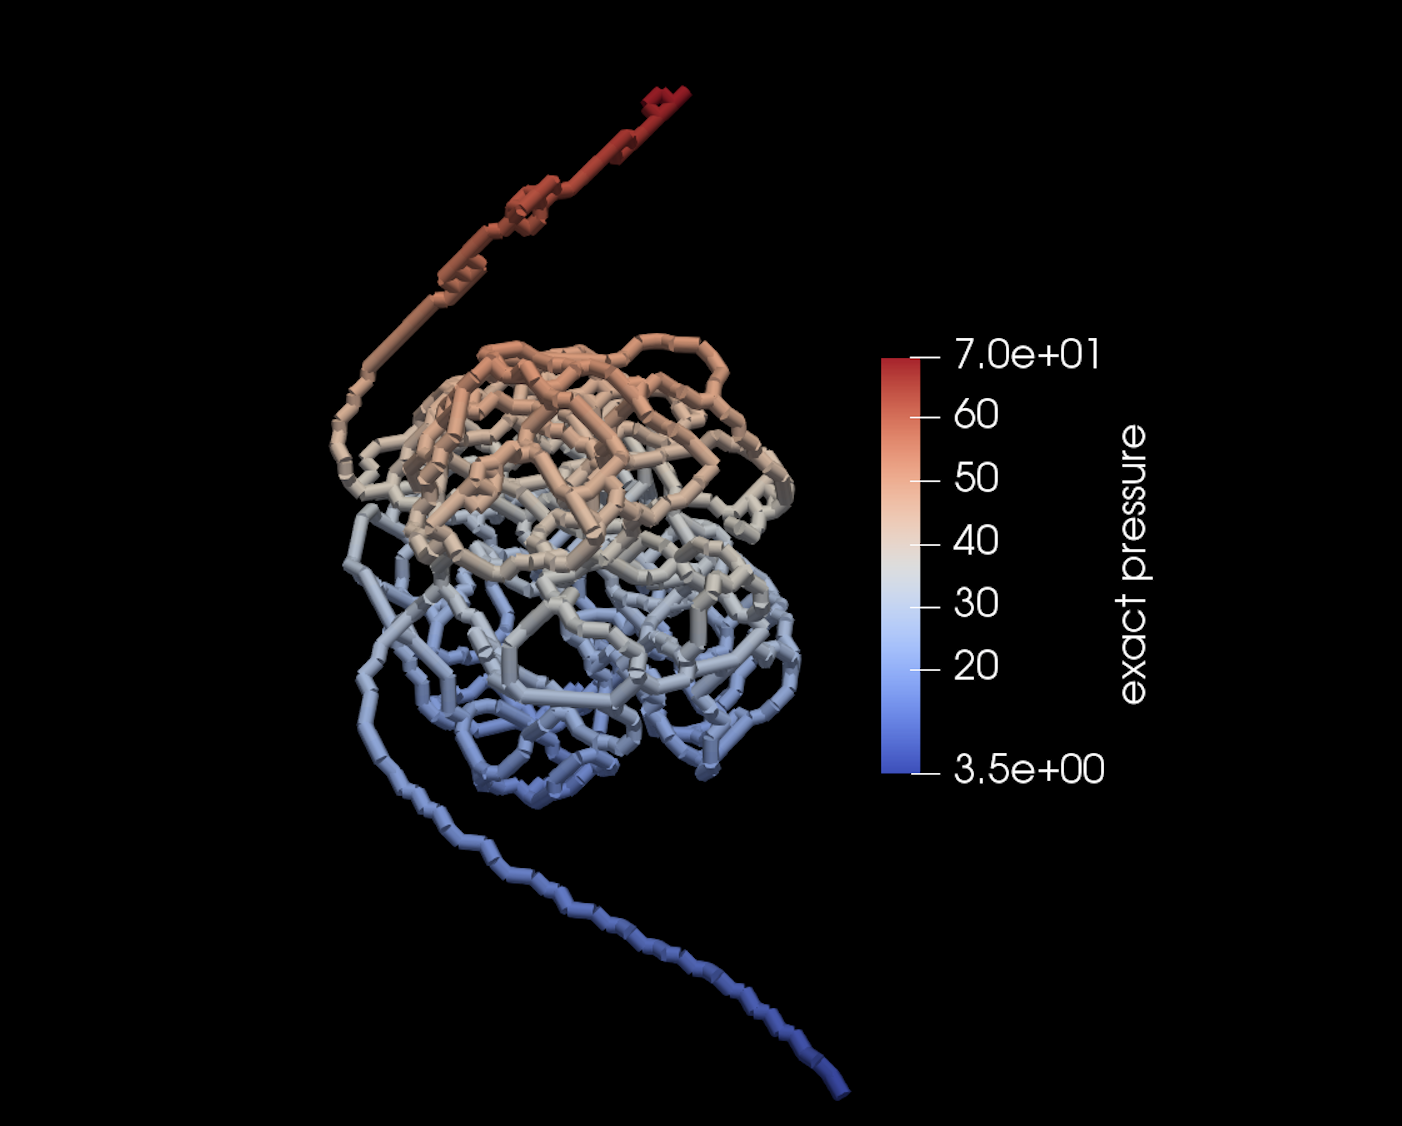
\includegraphics[width=162mm]{glom3_pressure}
\caption{Pressure Field in Glomerulus 3}
\label{fig:glom3_pressure}
\end{figure}
The figure \ref{fig:glom3_pressure} is the result of a DuMuX 1p-1p blood flow simulation computed on a Glomerulus network. The pressure field of the flow is visualized.\\

\begin{figure}[h]
\centering
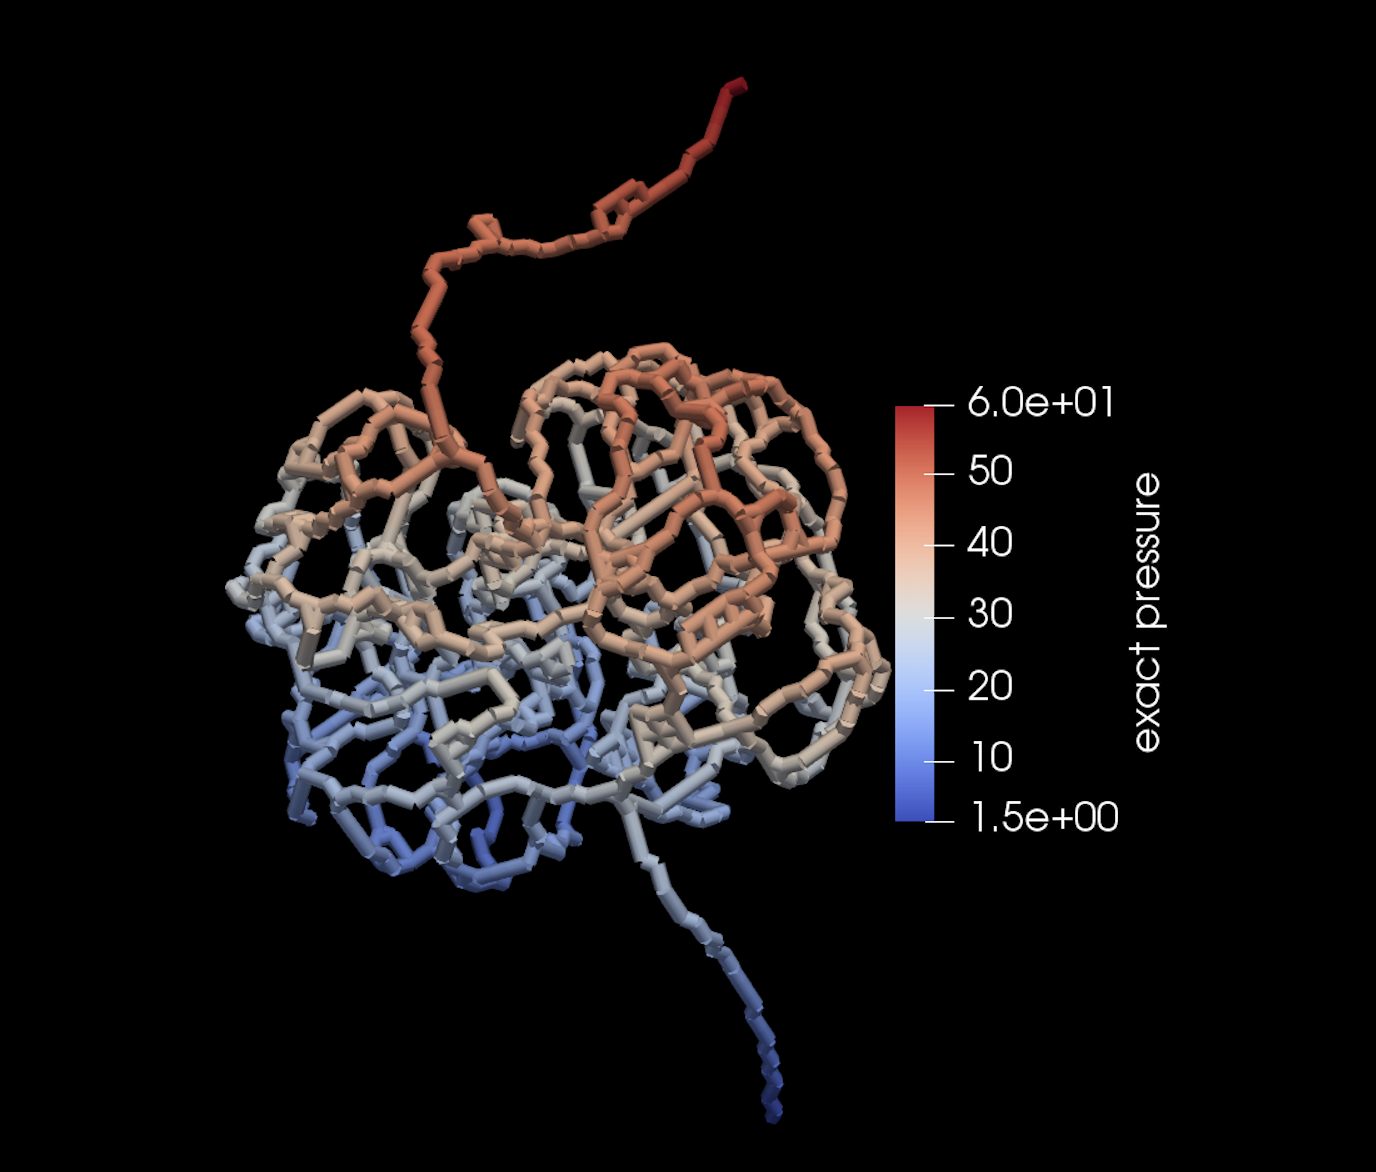
\includegraphics[width=162mm]{glom4_pressure}
\caption{Pressure Field in a Glomerulus 4}
\label{fig:glom4_pressure}
\end{figure}
The figure \ref{fig:glom4_pressure} is the result of a DuMuX 1p-1p blood flow simulation computed on a Glomerulus network. The pressure field of the flow is visualized.\\

\subsection{Comparison of the Results}
%Compare the produced results
In this section the main differences in the produced results by Green's Function Method and $DuMu^x$ for the same input files/same networks will be discussed.
\\General differences in terms of computational cost and implementation issues can be discussed here as well when explaining the differences in the results.
\\I might include the whole next section here, as this might be more compact.

%%%%%%%%%%%%%%%%%%%%%%%%%%%%%%%%%%%%%%%%%%%%%%%%%%
%\newpage
%\section{Comparison of the Different Methods Behind the Simulations}
%Compare DuMuX to Green's Method in general
%In this section the main differences between these two simulation methods described previously will be discussed.
%\\
%\\\textbf{Kartik do you think I need this 5th chapter at all ? I think I would rather delete it. I could include the subsections into the Simulation Methods part as well, and discuss some of these in the Conclusion as well ?}\\
%Compare the Solvers behind the Methods
%Very useful tu use Secomb Paper Numerical Methods section here
%\\In this section the main differences between the solvers and the associated numerical methods will be discussed.

%\subsection{Comparison of the Numerical Methods}
%Explain the Methods and differences between methods
%Very useful tu use Secomb Paper Numerical Methods section here
%In this section, the focus will be on comparing the numerical methods behind the Green's Method code and $DuMu^x$ and the differences in their implementation.

%\subsection{Stability Questions and Computational Cost}
%Explain when and why which the numerical methods are stable
%In this section, the consequences of the previously described differences will be discussed. The focus lies on the differences in terms of stability and computational cost for similar simulations.


\newpage
\section{Discussion}
%Summary of both methods in general and Outlook for the research field
%What this review was about: short summary. Main points
%highlighted. Perhaps a graph regrouping together elements.
%Comparison of different strategies and their state. Maybe your own
%thoughts on the whole story and where the promising directions lie
%and which ones you see with scepticism.

As seen previously, both the Green's Function Method and the implemented $DuMu^x$-based method can offer very interesting options. While the Green's Function Method is presenting a specifically created C++ based software for oxygen Transport and Diffusion simulations, the results show that the obtained outputs are not always satisfying (eventually will happen for new networks?). The reasons for this have been discussed previously (maybe repeat them shortly here).
Compared to this, the $DuMu^x$ based model is still in its very initial phase and cannot produce correct results yet (very probably). Still, the fact that it is $DuMu^x$ based offers both a large flexibility to the user in terms of further development, as well as in terms of computational flexibility when choosing a time- and space-discretization through choosing discretization modules and different grid creators. The solvers can also be chosen by the user, which doesn't guarantee an overall stable numerical solver, but can provide great flexibility when adapting the model to specific networks.
\\
\\As mentioned previously, one of the huge advantages of $DuMu^x$ is the flexibility it provides in terms of solvers, and thus in terms of the numerical methods used for the computations. This means that it is often possible to pick a solver which is stable for the specific problem and the chosen discretization.
\\
\\This is different for the Green's Method code, as there is no option of choosing a different solver than the one provided in the code. As discussed previously, this code is specifically implemented to solve and compute oxygen (or other Solute) concentrations in the blood and the surrounding tissue, and the implemented method strongly relies on the stability of the Green's Method and the numerical methods behind the solver.
\\
\\Main conclusions and final remarks.